\cleardoublepage

\section{研究相关技术概述}
本章将围绕本研究所涉及的核心技术展开介绍,包括扩散模型的基本原理与结构演进、跨模态特征融合策略,以及支撑长序列建模的时空位置编码方法。通过对这些关键技术的分析与整合,为后续提出的方法框架奠定理论基础与实践支撑。
\subsection{扩散模型}
视频扩散模型已经展示了从文本提示生成高质量视频片段的能力。这些模型(DiT模型)采用Transformer主干网络替代了传统的U-Net结构,从而在图像和视频生成任务中实现了更优的可扩展性。当前达到SOTA(State-of-the-Art,即当前最佳水平)的模型通常包含两个核心组件:一个用于时空压缩的变分自编码器 (Variational Autoencoder, VAE) 和一个用于序列化去噪的扩散Transformer,采用逐步去噪的方式生成符合要求的图像或视频。

\subsection{跨模态特征融合方法}
设计潜空间扩展策略,将参考图像特征沿时间维度进行动态扩展,通过可学习位置门控与目标序列进行深度融合。在Transformer架构中构建记忆增强机制, 通过不断计算参考图像和视频之间的相关性,实现身份特征的跨帧传播。此外在训练过程中每隔10个模块左右随机丢掉一些数据,使得相对于视频与参考图像不存在死板对应关系。同时在训练过程中强化生成序列与参考图像的特征空间紧致性,平衡外观一致性与运动自由度。

\subsection{时空位置编码系统}
将旋转位置编码扩展至三维时空域,通过建立帧间位置相对旋转矩阵建模运动连续性。使用分频编码策略,将低频分量分配至全局运动模式学习,高频分量聚焦局部细节时序对应,显著提升长序列生成稳定性。
\begin{equation}
R_{xyt} = R_x(\theta_i) \otimes R_y(\phi_j) \otimes R_t(\psi_k) 
\end{equation}
其中$\theta_i,\phi_j,\psi_k$分别对应空间坐标(i,j)和时间戳k的旋转角度。使用三维RoPE使得对于生成视频的动作质量和时空一致性方面有更明显的提升。

\subsection{本章小结}
本章围绕视频生成任务中的核心基本技术展开论述,重点介绍了视频扩散模型的架构演进、跨模态特征融合策略以及时空位置编码方法。在生成框架方面,基于Transformer主干的DiT替代传统U-Net,结合变分自编码器实现高质量视频生成。在跨模态融合部分,提出了结合参考图像的潜空间扩展机制和记忆增强模块,有效实现身份信息的时序传播与增强,提升了生成结果在外观一致性与运动自由度之间的平衡能力。同时,针对视频生成过程中的时空建模难点,设计了三维旋转位置编码系统,融合分频策略,显著提高了长序列生成的稳定性和时空一致性。这些方法共同推动了跨模态高质量视频生成模型在结构性与表现力上的全面提升。
\section{实验设计}
本章将从三个方面围绕参考图可控视频生成这一中心问题进行递进探讨,以增强生成视频的一致性,并且在保持生成质量的同时减少高分辨率参考图指导视频生成所需总时长。
\subsection{固定首帧的图像到视频生成}\label{sec1}
为了有效研究参考图像在引导视频生成过程中的作用,本章首先考虑一种将固定的参考图像作为视频序列首帧的参考图可控视频生成任务训练范式。

固定首帧的图像到视频生成框架的核心思想是将图像的静态信息显式地引入到视频动态内容的生成流程之初。通过这种方式,期望能够使模型在生成后续视频帧时,始终以参考图像的主题内容为基准,从而显著提升生成视频与输入图像在语义、风格及核心元素上的一致性。此举不仅有助于增强视频生成的准确性,亦能通过对参考图像的不同解读与动态演绎,促进生成内容的多样性。

在具体的模型实现中,一个关键步骤是对输入的参考图像进行高效表征。本章采用变分自编码器(VAE)将参考图像编码为其在潜在空间中的表示,即潜变量(latent variable)。将图像信息转换至潜变量空间进行处理,相较于直接操作像素空间,能够大幅降低数据维度,从而有效缩短模型训练时间、减少GPU显存消耗,并最终提升整体生成效率。

目前,在参考图可控视频生成任务的训练过程中,业界探索并应用了多种策略以融合参考图像信息。本章重点关注以下两种具有代表性的训练策略:

\textbf{首帧替换策略}:该策略的核心操作是将训练视频样本的第一帧,在潜变量层面,直接替换为参考图像经过VAE编码后的潜变量, 在经过DiT网络和真实视频直接进行相应Loss值计算通过梯度回传更新模型参数,以得到能够生成首帧主体人物细节的视频。具体细节见附录伪代码\ref{alg:first_frame_replacement}。值得注意的是,在每次训练迭代中,此参考图像的潜变量(记为 image\_latent)在输入后续的生成模型(如Transformer)时,不添加扩散模型通常所需的噪声。这样的设计确保了图像信息的纯净度。因此,在模型内部的注意力计算过程中,后续视频帧的表征(token)能够与这个无噪的图像信息进行充分交互。这种强引导使得模型从生成之初就严格依据参考图像的内容,从而确保生成的视频主题与图像内容高度相关,有效避免了主体漂移和人物失真等常见问题。
 

\begin{figure}[htbp]
    \centering
    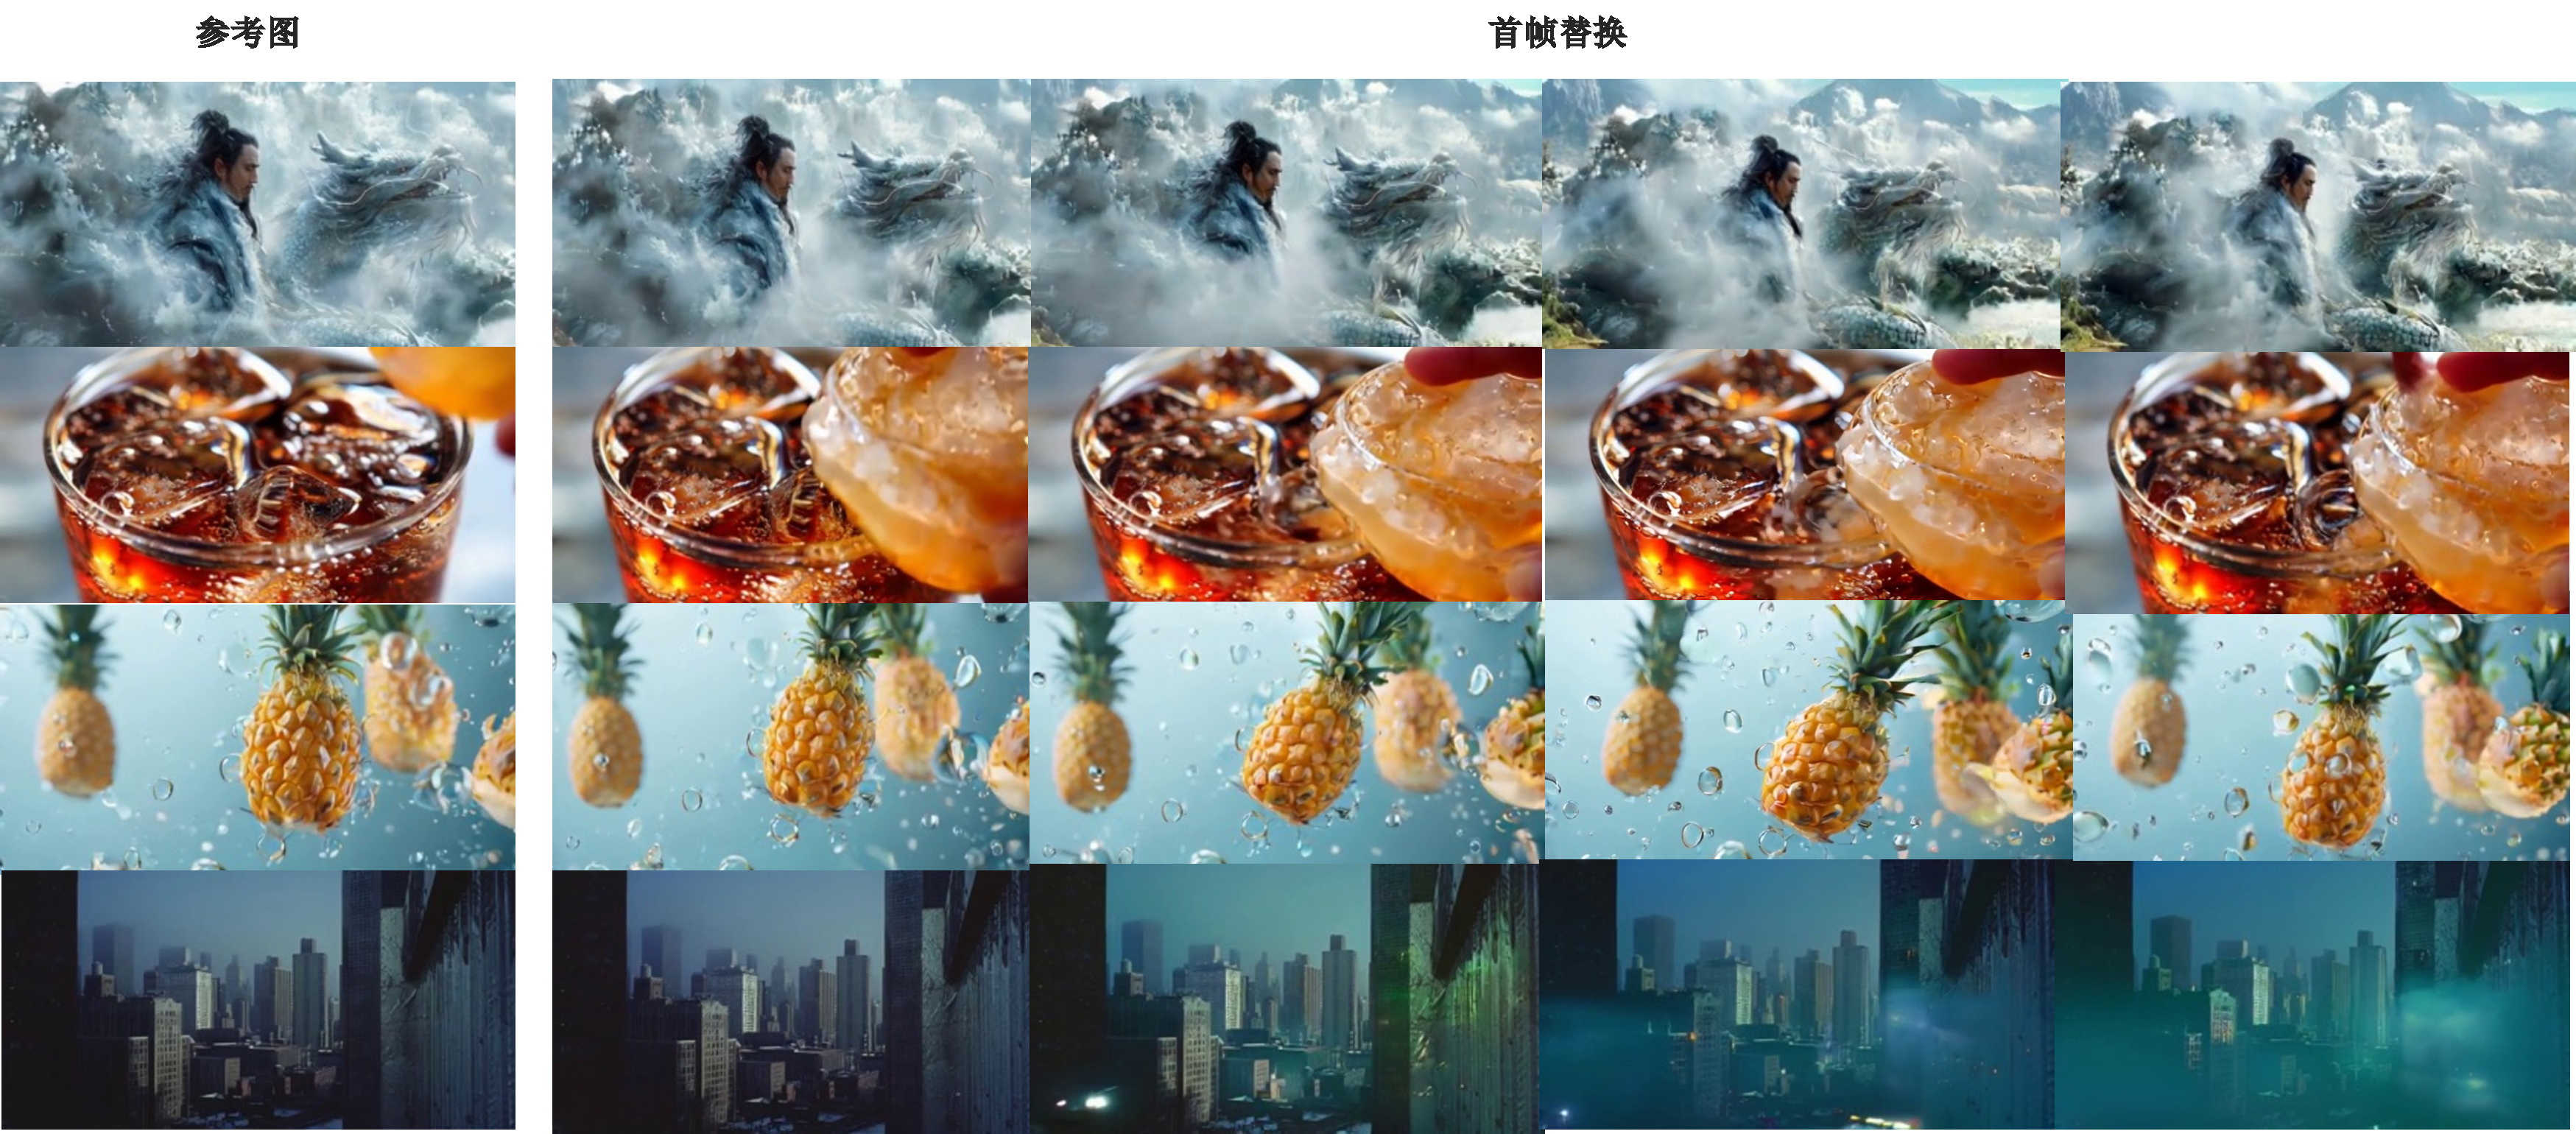
\includegraphics[width=0.8\textwidth]{final/I2V_1.pdf}
    \caption{\textbf{首帧替换策略生成结果示例}:图中展示了采用首帧替换策略生成的视频片段。可以看出,视频内容与首帧参考图像在主体特征上保持了良好的一致性。}
    \label{I2V_1}
\end{figure}

如图\ref{I2V_1}所示的生成案例,采用首帧替换策略能够产出基本符合预期的视频结果。视频中的主体一致性维持良好,未出现主体身份随时间演变而发生显著改变(主体漂移)或人物面部及形态出现不自然扭曲(人物失真)等不良现象。

\textbf{参考帧拼接策略}:与首帧替换策略不同,参考帧拼接策略将参考图像的信息融入视频生成过程的另一环节。具体而言,在训练时,参考图像的潜变量并非替换视频的首帧,而是与视频最后一帧的潜变量在时间维度上进行拼接。拼接后的序列随后被送入核心的Transformer模型进行序列建模和特征提取。


\begin{figure}[htbp]
\centering
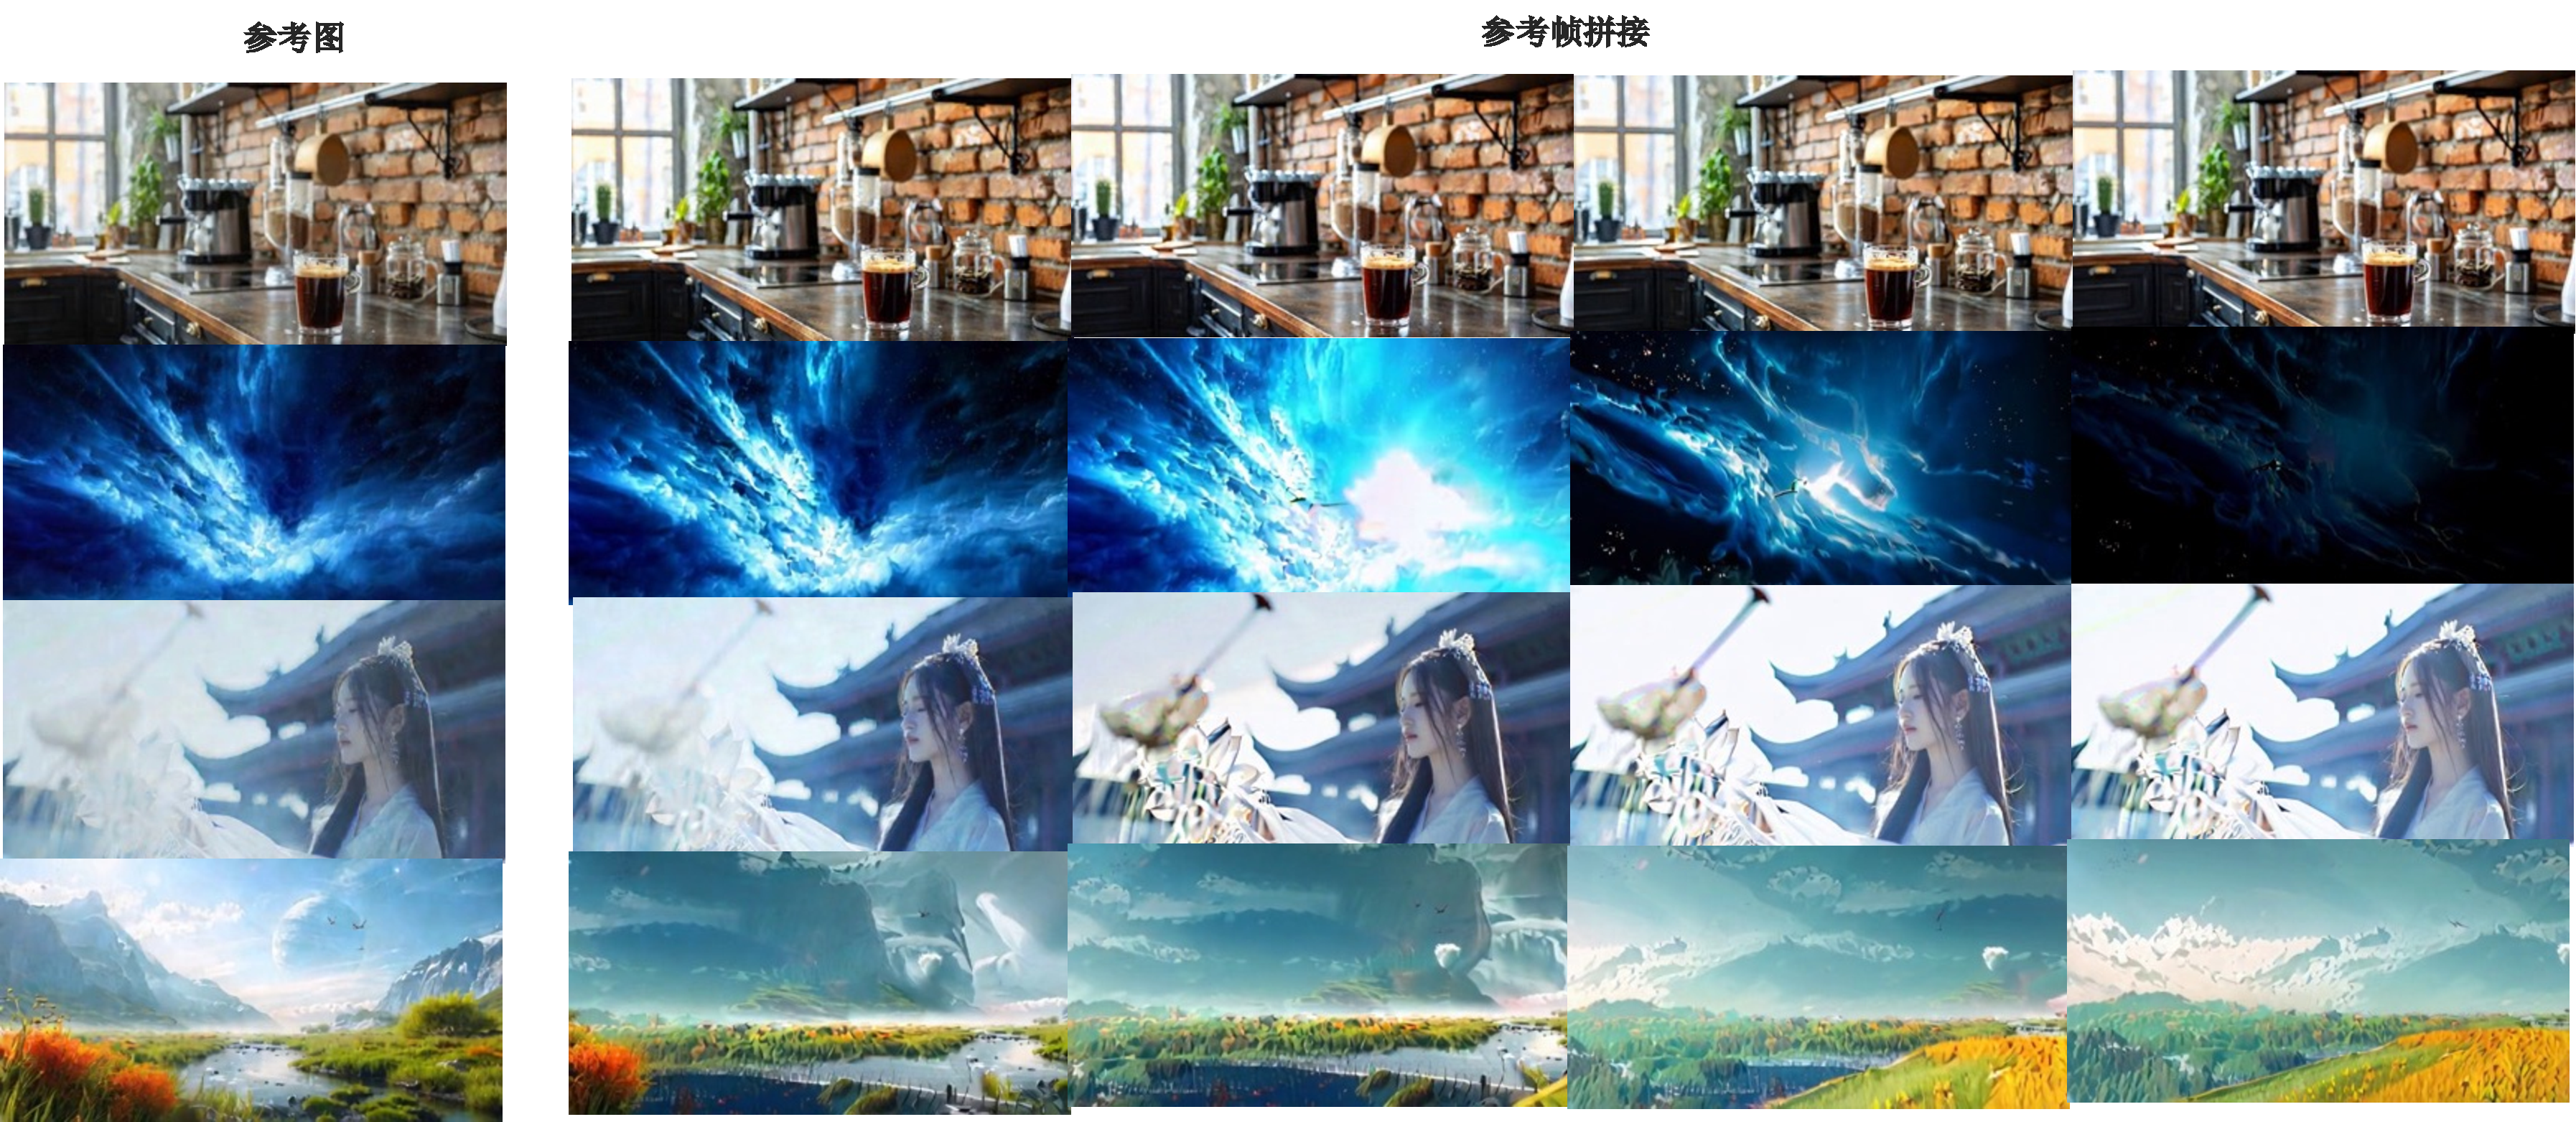
\includegraphics[width=0.8\textwidth]{final/I2V_2.pdf}
\caption{\textbf{参考帧拼接策略生成结果示例}:图中展示了采用参考帧拼接策略生成的视频。可见其在某些情况下运动幅度较小,但主体与参考图基本一致。}
\label{I2V_2}
\end{figure}
为了使模型能够区分正常的视频帧潜变量与作为参考信息的图像潜变量,需要在位置编码(positional encoding)阶段进行特殊处理。一种直接有效的方法是,将拼接在末尾的图像帧潜变量赋予与视频首帧相同的位置编码。通过这种方式,模型被引导将这个特殊的“最后一帧”识别为提供全局参考信息的图像,从而实现I2V的生成效果。\ 具体流程见伪代码\ref{alg:ref_frame_concat}。
此方法通过在时间序列的末端引入图像的全局视觉特征,期望模型在生成整个视频序列时都能参考这些特征,使得生成的视频能够更好地体现参考图像中的关键元素和整体风格。


从图\ref{I2V_2}的生成结果中可以观察到,参考帧拼接策略在某些案例上生成的视频运动幅度相对较小。例如,对于“女性手持花束并轻轻摇摆”的场景,视频中花束的摇动幅度可能不够显著。尽管如此,该策略依然能够保持生成视频中的主体人物或物体与参考图片内容基本一致。然而,其对于文本提示中描述动作的响应程度仍有提升空间。\\

\subsection{身份保持的视频生成}\label{sec2}

在探索了基于参考帧拼接的参考图可控视频生成策略之后,本章进一步思考如何在该框架基础上实现更灵活的身份(ID)信息保持。

本章尝试放开对拼接参考图像帧位置编码的特殊约束条件。即,本章将参考图像的潜变量直接拼接到视频序列潜变量的尾部进行训练,而不强制其位置编码与首帧相同, 具体流程见伪代码\ref{alg:id_injection}。\
本章期望通过这种方式,模型能够学习并提取参考图像中的核心ID信息(如人物的面部特征、物体的独特纹理等),并将其稳定地应用到生成的视频内容中。\
同时,由于摆脱了严格的位置编码模仿,本章希望生成的视频能够在保持ID一致性的前提下,展现出比原始参考帧拼接策略中观察到的更大幅度、更自然的动作,避免出现对参考图像姿态或动态的过度复刻现象。
\begin{figure}[H]
    \centering
    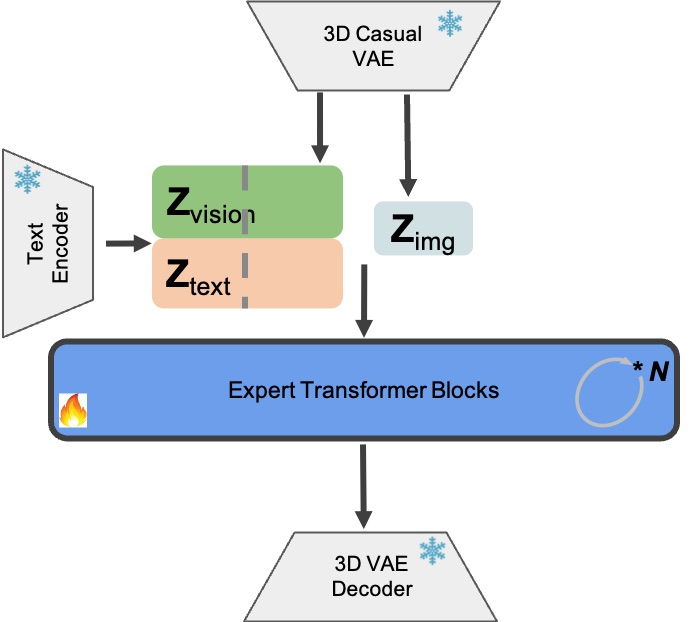
\includegraphics[width=0.8\textwidth]{data3.pdf}
    \caption{\textbf{基于DiT的参考图像引导视频生成之图像帧拼接策略框架图}:流程显示图像经VAE编码为潜变量,与其他数据结合后输入专家Transformer模块处理,最终解码输出视频。}
    \label{architecture1}
\end{figure}
本章中ID保持视频生成方法所采用的基础框架如图\ref{architecture1}所示,该框架基于DiT(Diffusion Transformer)结构进行构建。特别的目前无论是图像领域\cite{peebles2023scalable,chen2023pixart} 还是视频领域~\cite{hong2022cogvideo, yang2024cogvideox, kong2024hunyuanvideo, lin2024open}都证明了DiT模型生成效果要显著优于UNet模型。\
其核心流程如下:首先,输入的参考图像通过一个VAE编码器被转换为低维的潜在空间表示(latent space)。随后,该图像潜变量与其他数据(例如,文本提示的嵌入表示,或视频中其他帧的潜变量)进行有效结合(例如,通过拼接操作)。整合后的信息被送入一个或多个专家Transformer模块(Expert Transformer modules)进行深层次的特征提取和序列建模。Transformer模块通过其自注意力机制,能够有效地捕捉不同信息源之间的复杂依赖关系,并学习从参考图像ID到动态视频内容的映射。最后,经过Transformer处理的序列潜变量通过一个VAE解码器,被还原为像素空间的视频帧序列,从而完成视频的生成。

% \subsection{本章小结}
% 基于上述两个章节(固定首帧的图像到视频生成,身份保持的视频生成),本章尝试参考帧拼接策略、首帧替换、ID注入方式来完成参考图可控视频一致性生成任务,并且在一定程度上解决了原本视频生成的视频主体漂移,一致性保持程度不佳等问题。在生成视频的背景一致性、运动流畅性、动态程度、美学质量和图像质量方面取得了一定成果。

\subsection{高分辨率参考图视频生成}
通过前两部分的探索,本章已经能够实现生成视频在保持参考图像基本主体信息方面的较好效果。然而,这些实验主要在中低分辨率下进行。当给定一个高分辨率(如720p、1080p甚至2K)图片,本章希望生成和图片分辨率一致的高分辨率视频时,囿于现有模型(尤其是基于扩散的模型)的固有计算复杂度,单张参考图引导的高分辨率视频生成会耗费大量的计算时间和显存资源。为了解决这一瓶颈,本章参考了Zhang等人提出的FlashVideo\cite{zhang2025flashvideo}工作,选择采用一种基于流匹配(flow matching)的方式来高效生成高分辨率视频。

\begin{figure}[htbp]
    \centering
    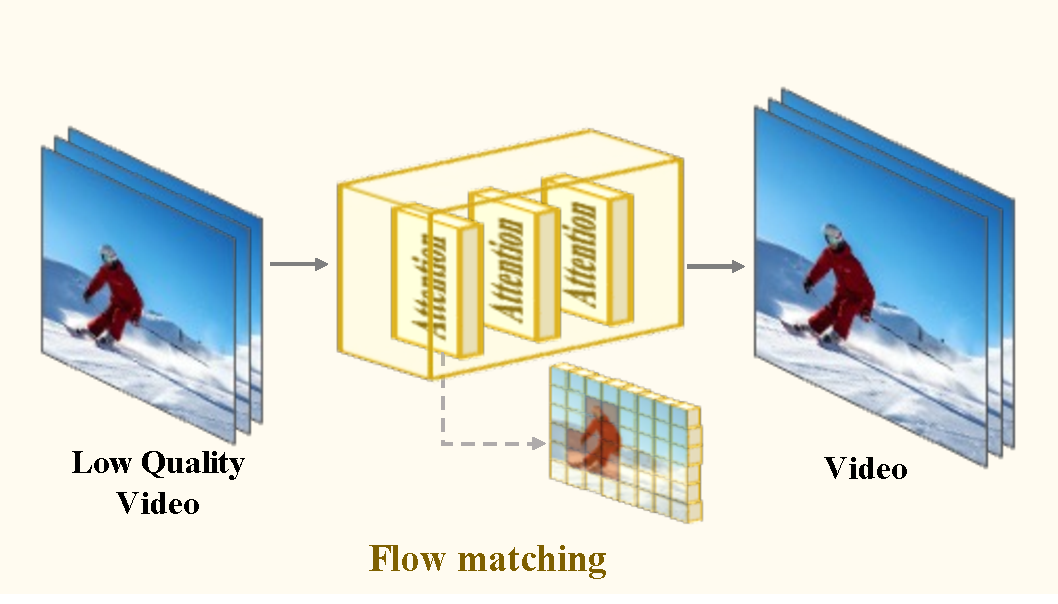
\includegraphics[width=0.8\textwidth]{final/pipeline3.pdf}
    \caption{\textbf{本章基于DiT模型来实施flowmatching方法}
    }
    \label{fig:flowmatching}
\end{figure}
为显著减轻高分辨率视频生成中的计算开销,本章提出了\textbf{基于流匹配的高效生成方法}。本章采用了一个参数量为10亿(1B)的轻量级流预训练模型。该模型的核心优势在于能够提高每一步去噪(或在此处理解为生成)的效率,具体性能数据如后续表\ref{tab:time_size}所示。\
该方法在初始化阶段消除了传统扩散模型中冗余的采样步骤,并且避免了对额外复杂控制参数(如分类器指导权重)的依赖。
在推理(生成)过程中,本章首先从一个低分辨率的潜变量 $\mathbf{lr\_latent}$ (由低分辨率视频或图像编码得到) 开始。为了增强模型的生成能力并避免对 $\mathbf{lr\_latent}$ 内容的过度依赖(从而允许更多的生成多样性),本章向 $\mathbf{lr\_latent}$ 中注入一定量的噪声。此退化(或称扰动)过程可定义为:
$z_1 = \alpha \cdot \mathbf{lr\_latent} + (1 - \alpha) \cdot \text{noise}, \quad \text{其中} \ \text{noise} \sim \mathcal{N}(0, \mathbf{I})$
这里$z_1$代表了起始的、略带噪声的低分辨率潜变量,$\alpha$ 是一个平衡因子,$\mathcal{N}(0, \mathbf{I})$ 表示标准正态分布的噪声。
然后,本章通过一个基于常微分方程(ODE)的积分方法,沿着$n$个离散时间步$t_{i=0}^n$对该潜变量进行迭代优化,将其逐步逼近为高分辨率视频的潜变量。这一过程可以形式化表示为:
\[\
z_1 = z_0 + \sum_{i=0}^{n-1} u_\theta(z_{t_i}, t_i) \cdot (t_{i+1} - t_i)
\]\
其中$z_0$是目标(高分辨率)潜变量(在训练阶段)或前一步的潜变量(在推理阶段),$u_\theta(z_{t_i}, t_i)$是由参数为$\theta$的神经网络在时间$t_i$和状态$z_{t_i}$下预测的速度场,也可以直观理解为希望模型预测的方向。
在训练过程中,本章定义了$z_0$和$z_1$之间的线性插值轨迹:
$z_t = (1 - t) z_0 + t_{z_1}, \quad t \in [0,1]$
该轨迹描述了从 $z_0$ 到 $z_1$ 的直接路径。对应的真实速度场(即 $z_t$ 关于 $t$ 的导数)则由下式给出:\[\ 
u_{t,\theta} = \frac{dz_t}{dt} = z_1 - z_0
\]\



为了建立$\mathbf{lr\_latent}$和$\mathbf{hr\_latent}$之间的配对关系,本章将上述定义中的 $z_0$替换为目标高分辨率潜变量$\mathbf{hr\_latent}$,并将$z_1$替换为输入的低分辨率潜变量$\mathbf{lr\_latent}$。训练的目标是让流匹配模型能够学习到从$\mathbf{lr\_latent}$到$\mathbf{hr\_latent}$的方向信息,\
这样,在推理时,模型就能够在少数几个步骤内,有效地将低分辨率信息引导并转换为高质量的高分辨率视频。


具体而言,在推理(生成高分辨率视频)过程中,本章从$z_1$出发并根据模型预测的速度场$u_{t,\theta}$进行迭代更新,以逐步接近目标的高分辨率表示:
\[\ 
z_1 \leftarrow z_1 - \text{dts}[i] \cdot u_{t,\theta}
\]\, 其中$\text{dts}[i]$代表第$i$个积分步长$(t_{i+1} - t_{i})$。
而在建立了上述理论分析认知基础上,整个模型的训练就显得十分直接。只需要同时输入低质量视频和高质量视频,不断让低质量视频逼近高质量视频即可。本章对此作出简单示意图\ref{fig:flowmatching}。

\subsection{本章小结}
本章聚焦于解决参考图可控视频生成的核心问题,提出并设计了一系列实验。围绕增强生成视频一致性和优化高分辨率生成效率,循序渐进地介绍了本文的主要实验设计和训练流程,并在附录中提供了相应的伪代码以方便理解和复现。具体研究内容包括对固定首帧图像到视频生成的两种不同训练策略(首帧替换和参考帧拼接)的对比分析;基于类似参考帧拼接思想,实现更灵活的身份(ID)信息保持的视频生成方法;以及为显著降低高分辨率视频生成计算开销而提出的基于流匹配的高效生成方法。
\section{实验结果与分析}
\subsection{评估方法}

为更好地评估生成视频的质量,本章从定性与定量两个维度,对不同设置下的实验结果进行了多方面分析,并构建了一个包含108个文本提示词的测试集,涵盖人物、动物、物体和风景等多种类别,提示词来源为opensora和VBench的官方文本提示词。本文使用VBench这一公开的视频生成质量评估基准进行了定量测量。\
VBench从主体一致性,背景一致性,运动平滑度,动态程度,美学质量和图像质量这六个维度用自动化评估的方式对于文本生成视频(Text-to-Video)任务进行评估。具体而言:

(1)主体一致性主要是衡量视频中主体(如人物、动物、物体等)在整个视频帧序列中的外观一致性,通过DINO计算视频语意信息。

(2)背景一致性主要是衡量背景在时间维度上的稳定性,避免抖动、漂移或不连贯变动,使用 CLIP 计算帧间相似度。

(3)运动平滑度主要是衡量视频中物体运动是否自然、平滑,无跳帧或抖动,通过评估光流向量在时间上的平稳程度来体现物体运动情况。

(4)动态程度主要是衡量频中的运动量大小,是否具备真实世界中常见的动态变化,通过光流平均值来衡量运动强度。

(5)美学质量主要是衡量视频画面的审美质量,如构图、色彩、光影等,通过LAION美学预测器模型来进行评估生成视频美感。

(6) 图像质量主要是衡量图像的清晰度、去噪程度、是否存在压缩伪影等问题,通过MUSIQ多场景图像质量评分网络来评估生成图像美感。

此外,为了增加实验结果可靠性,本章还使用了包括针对单帧图像质量的MUSIQ\cite{ke2021musiq}、MANIQ\cite{maniqa}(和NIQE\cite{niqe},以及针对视频整体质量的DOVER\cite{dover}评价体系中的技术质量(Tech)和美学质量(Aesthetic)
对于生成结果进行补充评估。MUSIQ是一种基于多尺度视觉建模的无参考图像质量评价模型,通过输出一个连续的图像质量得分,反映其主观视觉质量;\
MANIQA通过融合多维注意力机制用于高质量图像生成效果评价;NIQE通过分析自然图像的统计分布特征,来评估图像生成质量;DOVER 是一种新近提出的视频质量评估体系,可从时间一致性、视频清晰度与主观美感等多维度对视频进行评估。
% 在训练中,本文发现针对拼接策略直接训练

\subsection{参考图可控视频生成方法效果评估}
针对固定首帧的图像到视频生成的两种参考图可控视频生成训练策略的性能差异,本章进行了一系列对比实验。如图\ref{I2V_4}和图\ref{I2V_3}所示,本章选取了若干具有代表性的文本提示(prompts)进行测试,这些提示涵盖了不同场景、主体和动作。

例如,对于文本提示:
\begin{figure}[htbp]
    \centering
    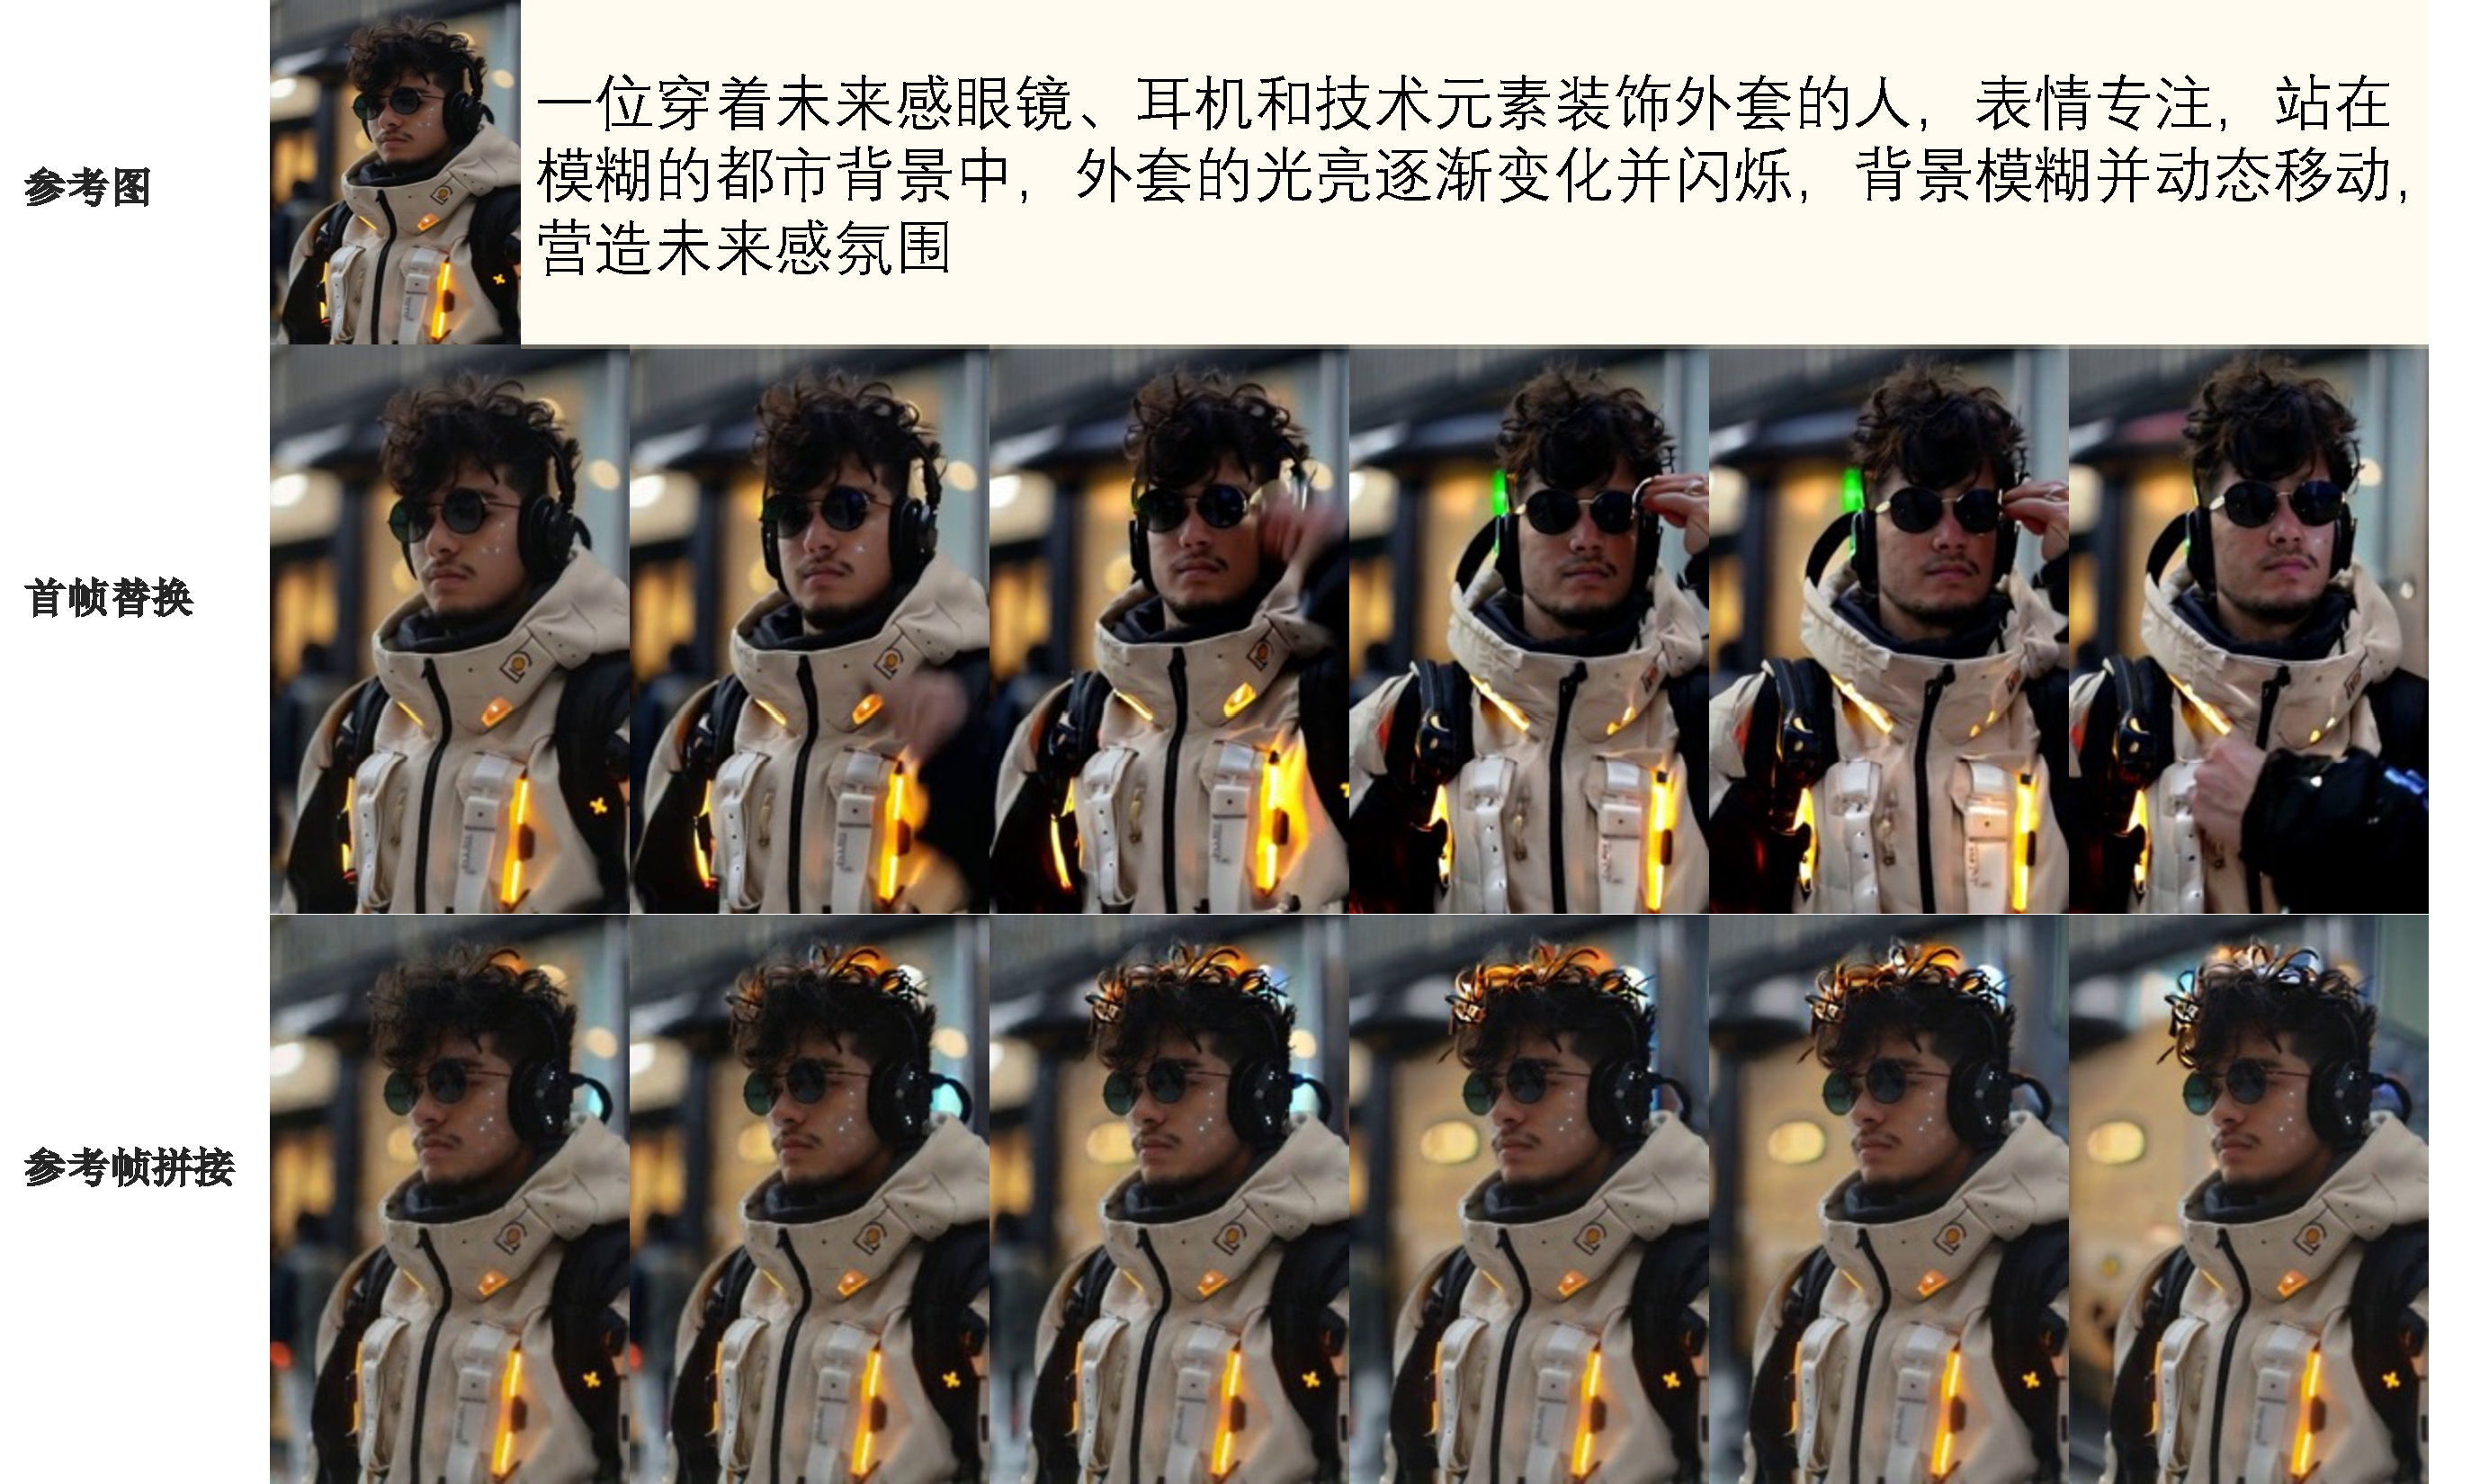
\includegraphics[width=0.8\textwidth]{final/I2V_4.pdf}
    \caption{\textbf{两种不同训练策略生成结果对比 (一)}}
    \label{I2V_4}
    \end{figure}
\begin{itemize}
\item Red-eyed woman in snow with serene and mysterious atmosphere, melting snow (一位红瞳银发的女性置身雪境,衣帽上附着雪花,氛围宁静而神秘,雪渐消融)。
\item Man with long hair in traditional attire emerges from mist with a serpent-like creature (一位身着传统服饰的长发男子携蛇形生物自雾气中显现)。
\item Glass with brown drink and ice cubes, spilling as more ice is added (一杯盛有棕色饮品与冰块的玻璃杯,因继续加入冰块致使饮品溢出)。
\item Pineapples floating and rotating in water, surrounded by rising bubbles. (菠萝在水中悬浮并缓慢旋转,周遭气泡氤氲上升,营造宁静氛围)。
\end{itemize}


\begin{figure}[htbp]
    \centering
    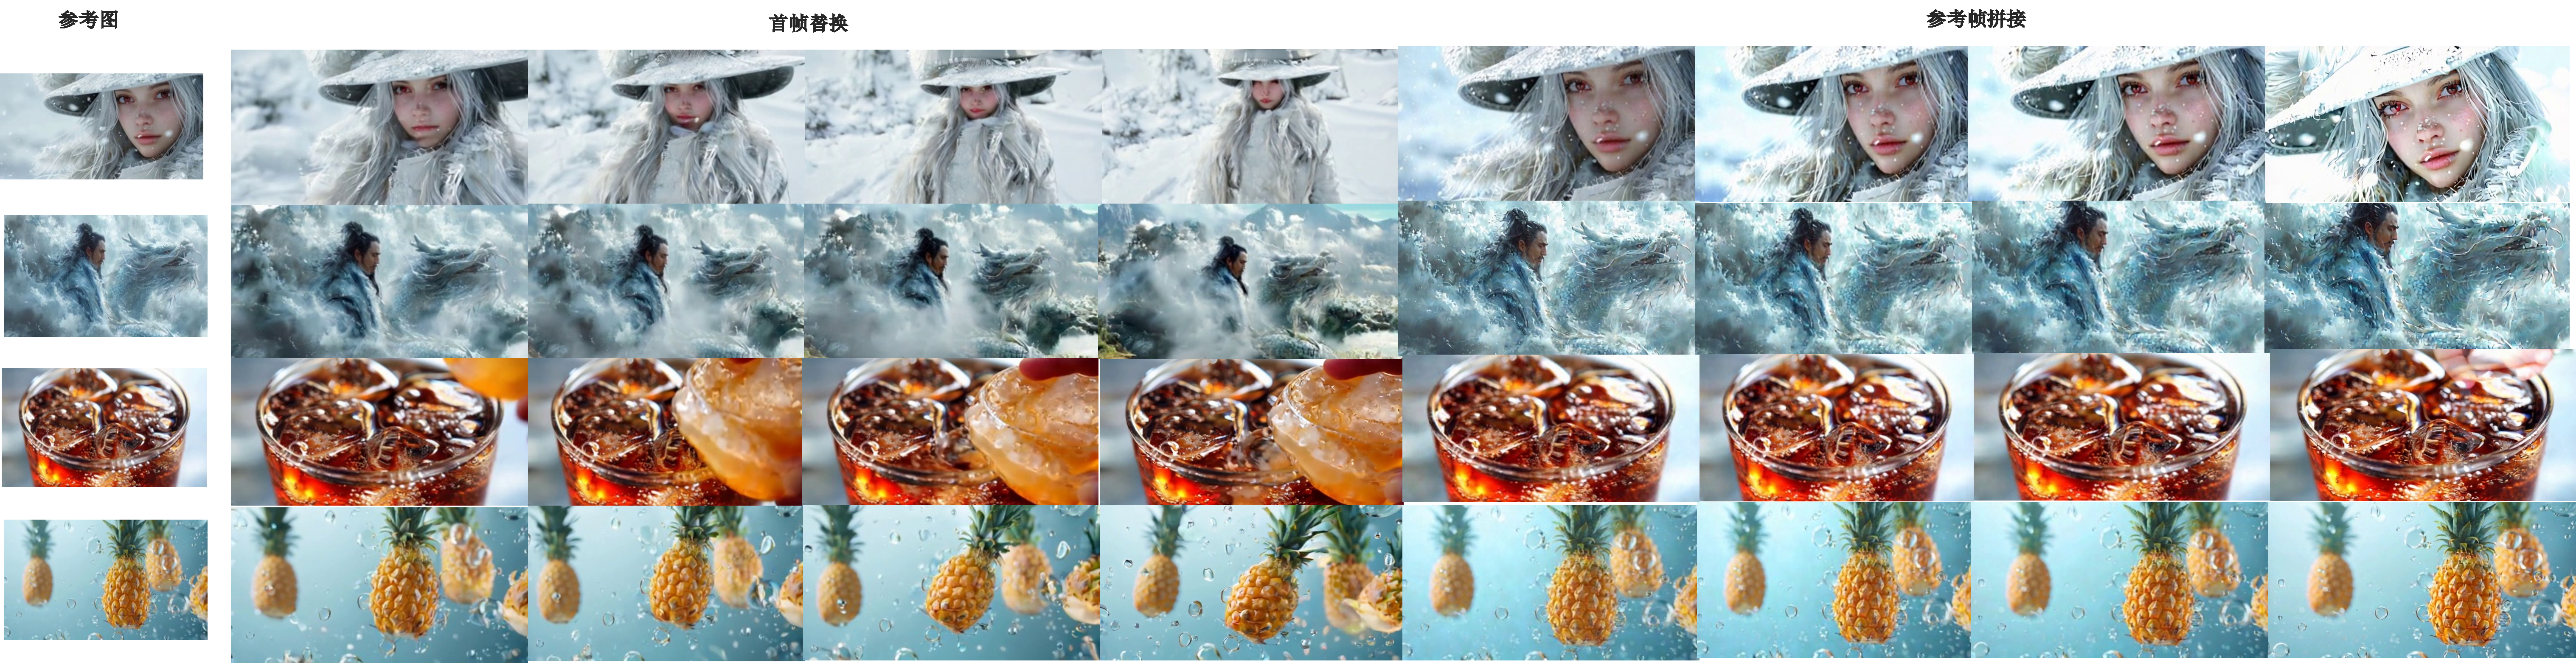
\includegraphics[width=0.8\textwidth]{final/I2V_3.pdf}
    \caption{\textbf{两种不同训练策略生成结果对比 (二)}}
    \label{I2V_3}
\end{figure}

通过对图\ref{I2V_4}和图\ref{I2V_3}中的生成结果进行细致观察与比较,可以明显发现,首帧潜变量替换策略生成的视频在动作幅度上通常大于参考帧潜变量拼接策略。此外,在语义保持度方面,首帧替换策略也表现更优。例如,当文本提示要求菠萝做出“摇滚动作”时,首帧替换策略生成的视频能够更充分地满足这一略带夸张的语义要求,展现出更强的动态性和文本遵循能力。

值得一提的是,作者在实验过程中还观察到,首帧替换策略的训练收敛速度通常快于参考帧拼接策略。根据经验,参考帧拼接策略达到相似训练效果所需的梯度迭代次数(或训练时长)约为首帧替换策略的两倍。

综上分析,考虑到生成效果的动态性、语义一致性以及训练效率,在后续章节探讨高分辨率参考图可控视频生成生成任务时,本文将优先选用并基于首帧潜变量替换策略进行进一步的研究与优化。

\begin{figure}[htbp]
    \centering
    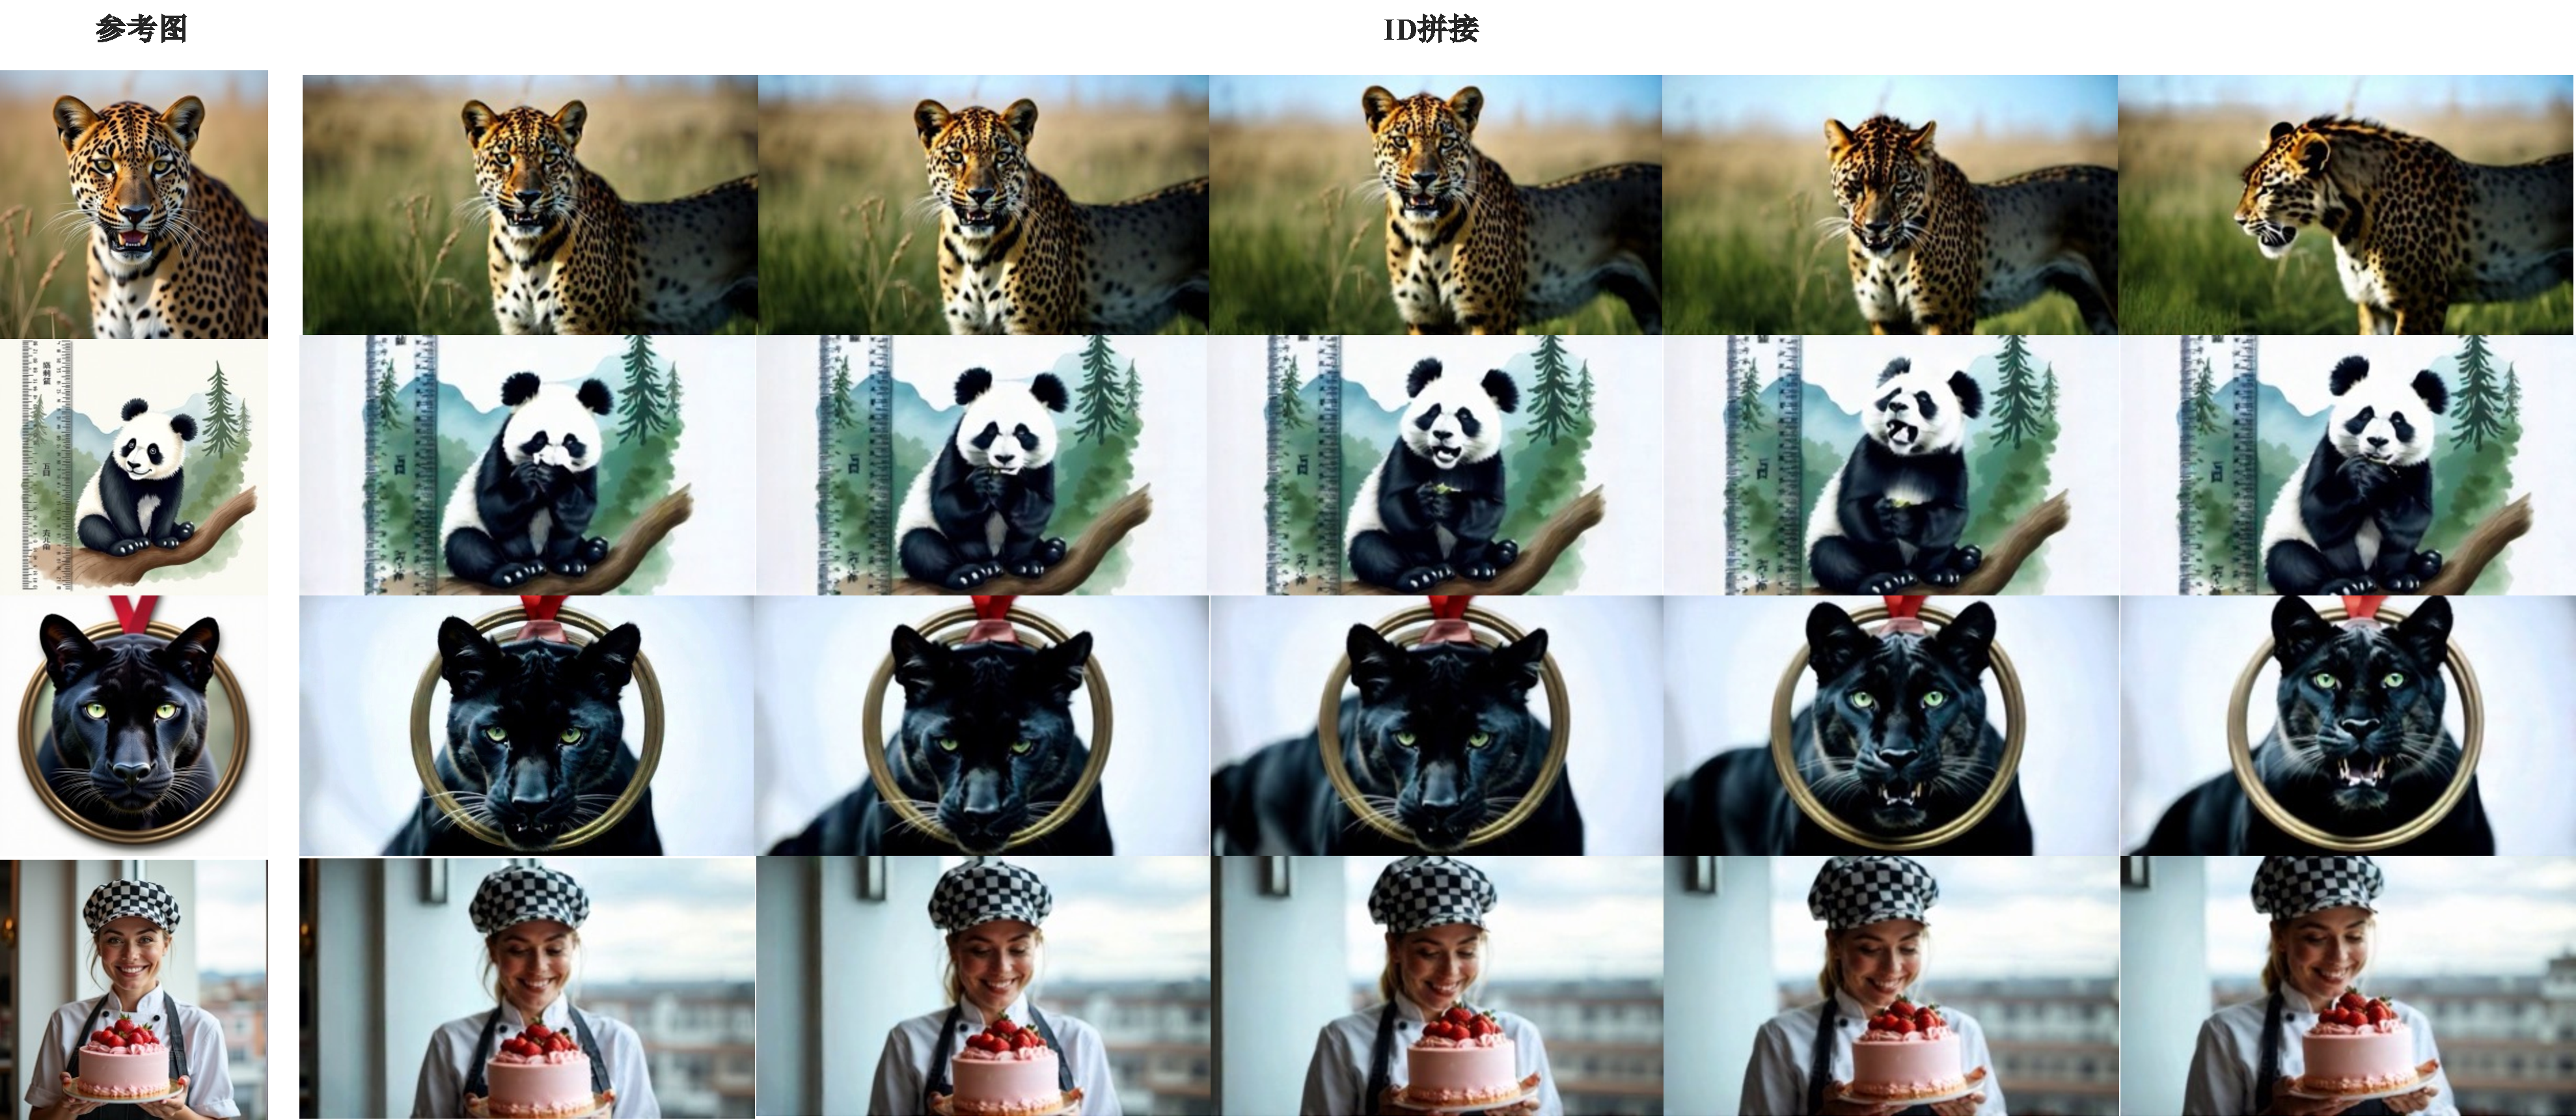
\includegraphics[width=0.8\textwidth]{final/IDconcate_2.pdf}
    \caption{\textbf{注入ID信息的视频生成结果 (多样化场景案例)}:展示了动物和人物主体下的ID保持与动态生成效果。}
    \label{IDconcate_2}
\end{figure}


为了验证所提出ID保持视频生成方法的有效性,本章进行了一系列实验,选用了包含不同动物和人物的案例作为测试。

如图\ref{IDconcate_2}所示,本章展示了针对豹子、熊猫、黑豹以及一位头戴厨师帽的女性等不同主体的生成结果。在这些视频中,各主体均表现出了其独特的个体特征,表明模型成功捕捉并维持了参考图像中的ID信息。同时,视频内容也展现了相应的视觉变化和动态效果,确保了在不同场景或动作下,生成内容仍能维持一致的身份特征。这证明了该方法在平衡ID保真度与视频动态性方面的潜力。

本章进一步考察了该方法在更多样化场景下的表现。如图\ref{IDconcate_1}所示的第一组图像集合,包含了色彩鲜艳的鱼类、身着急救人员制服的人物以及群体活动等不同场景。从生成结果来看,视频的动作和运动状态较好地响应了相应的文本提示,展现了良好的动态性。并且,每个视频都围绕特定的主题进行生成,在保持人物或场景核心元素随时间发生合理变动的同时,确保了生成的主体内容与给定参考图像的元素特征保持一致。

此外,针对文本描述中包含更大幅度动作(如飞驰、跳舞、做技巧动作等)的情况,本章也进行了相应的实验验证,结果如图\ref{IDconcate_3}所示。对应的文本提示词包括:

\begin{figure}[htbp]
    \centering
    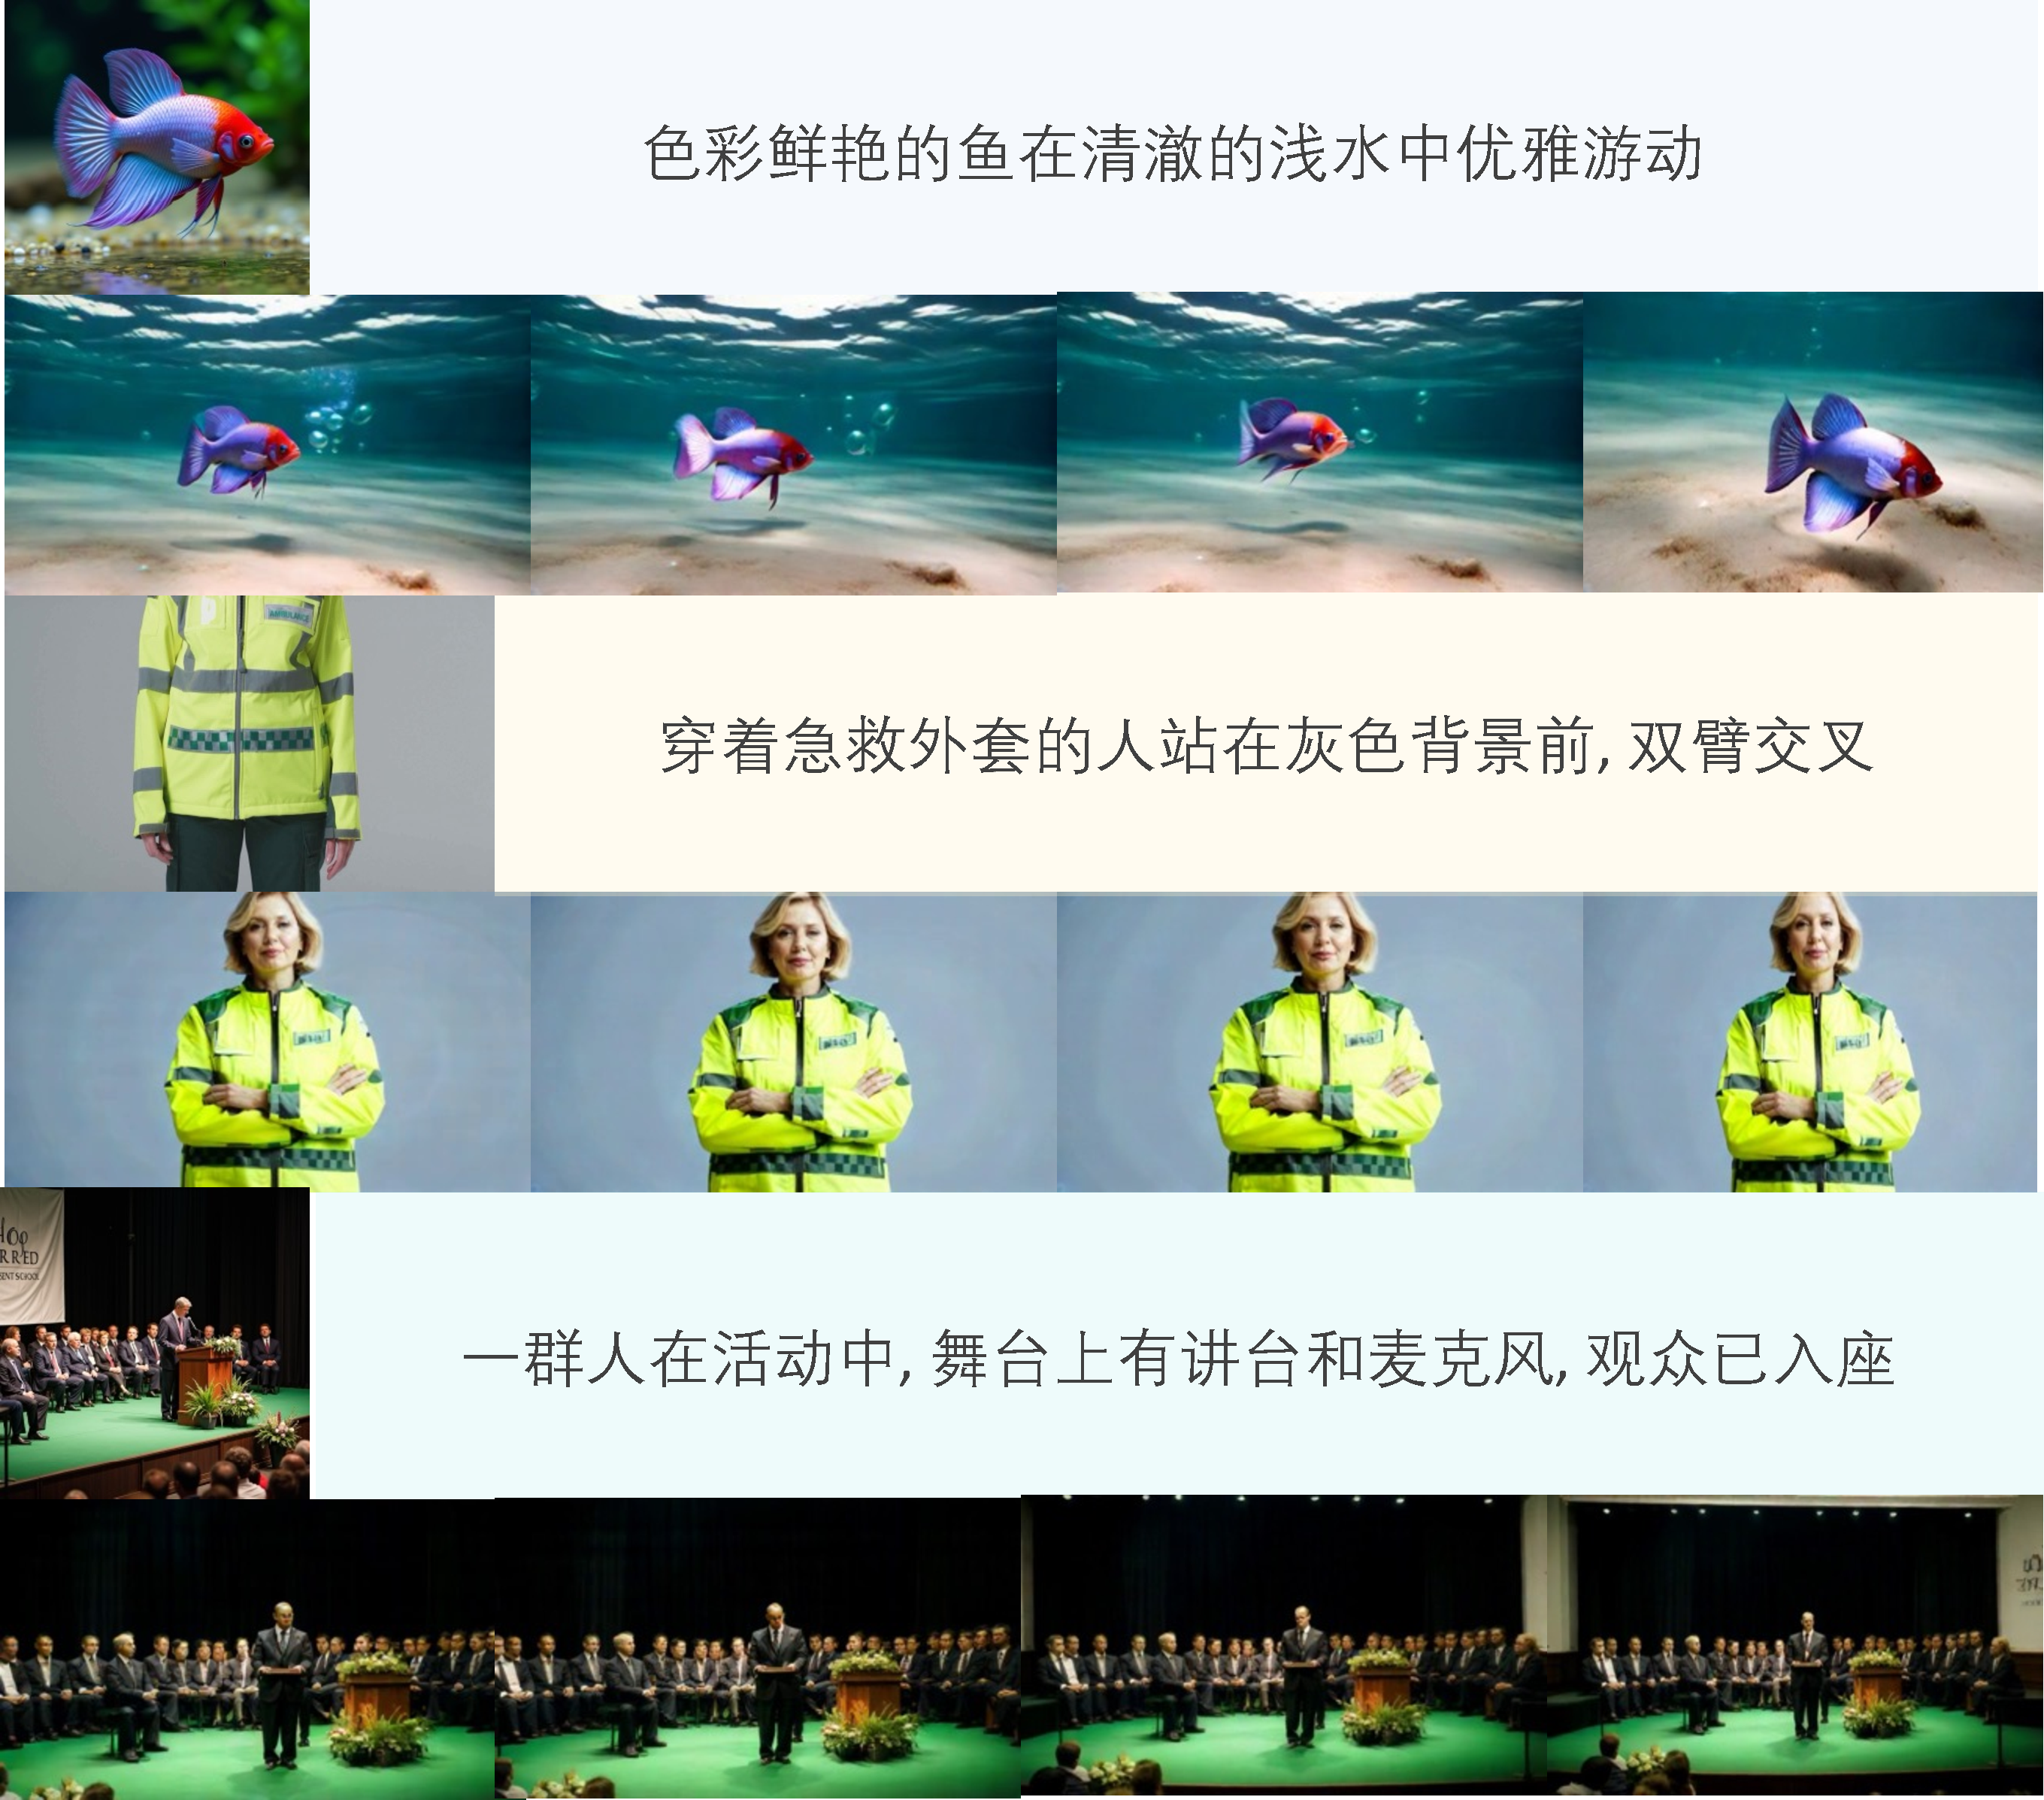
\includegraphics[width=0.8\textwidth]{final/IDconcate_1.pdf}
    \caption{\textbf{注入ID信息的视频生成结果 (多样化场景案例)}:展示了在鱼、急救人员及群体活动等场景下的ID保持与动态生成效果。}
    \label{IDconcate_1}
\end{figure}

\begin{itemize}
\item Red sports car speeding through rain, tires splashing in wet street. (一辆红色跑车在大雨中飞驰,轮胎溅起水花,快速行驶在湿滑的街道上。)
\item Whimsical girl with curly hair and wings dancing with pinwheel among flowers. (一位异想天开、拥有卷发和翅膀的女孩,在花丛中手持风车欢快地跳舞。)
\item Skateboarder performing mid-air trick against bright blue sky and sun. (滑板爱好者在明亮的蓝天与阳光背景下,于空中做出技巧动作。)
\end{itemize}
从图中可以看出,即使对于这些高动态的场景描述,生成的视频在文本响应度方面也表现较为良好,ID信息得到了有效维持,同时动作的流畅性和合理性也得到了保证。

\begin{figure}[htbp]
    \centering
    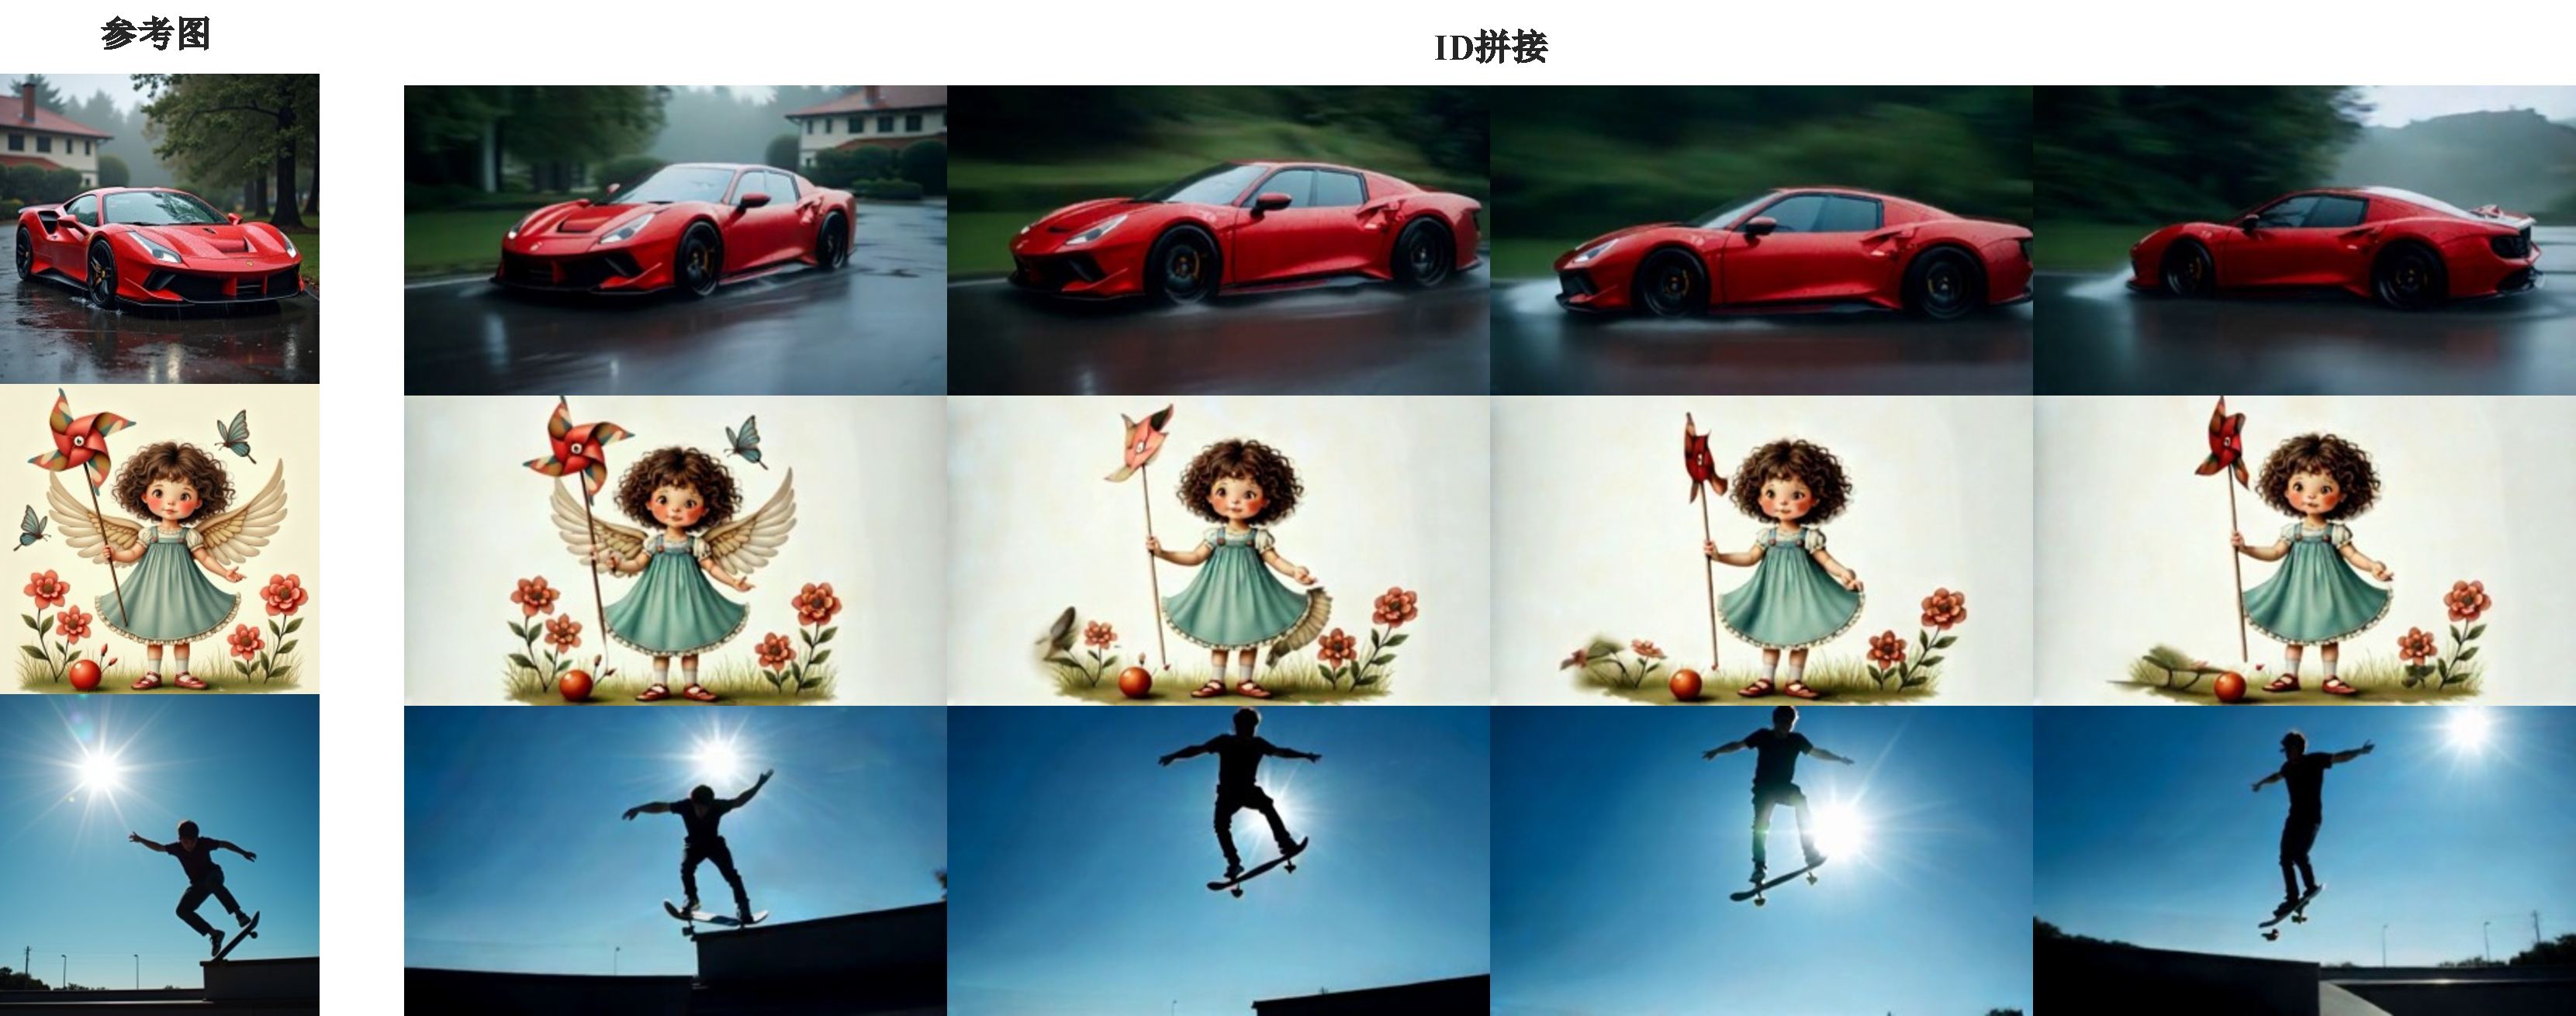
\includegraphics[width=0.8\textwidth]{final/IDconcate_3.pdf}
    \caption{\textbf{注入ID信息的视频生成结果 (大幅度动作案例)}:展示了在飞驰、跳舞和滑板技巧等高动态场景下的ID保持与文本响应效果。}
    \label{IDconcate_3}
\end{figure}

为了更客观地评价所提出的ID注入方法以及前述其他参考图可控视频生成策略的性能,本章采用了VBench\cite{huang2023vbench,huang2024vbench++,zheng2025vbench2}指标进行评测。本章的评估结果如表\ref{tab:vbench}所示,对于每个指标作者采用测试五遍取平均值方法以确保结果的合理性。

\begin{table*}[t]
\centering
\caption{不同方法在VBench各项指标上的表现对比}
\scriptsize
\setlength{\tabcolsep}{2pt}
\renewcommand{\arraystretch}{1.0}
\resizebox{1\textwidth}{!}{
\begin{tabular}{l|c|c|c|c|c|c}
\toprule
\textbf{方法} & \textbf{主体一致性} & \textbf{背景一致性} & \textbf{运动平滑度} & \textbf{动态程度} & \textbf{美学质量} & \textbf{图像质量} \\
\midrule
Wan视频 \cite{wan2025} & 92.83 & 95.42 & 98.47 & 54.84 & 62.66 & 69.04 \\
参考帧拼接 (Reference-Frame Concatenation) & 93.12 & 95.88 & 98.09 & 45.45 & 62.40 & 62.70 \\
首帧替换 (First-Frame Replacement) & 89.22 & 93.53 & 98.81 & 63.64 & 58.25 & 58.09 \\
\textbf{ID注入 (ID Injection)} & 95.76 & 95.80 & 99.30 & 37.29 & 57.19 & 58.15 \\
\bottomrule
\end{tabular}
}
\vspace{-0.1in}
\label{tab:vbench}
\end{table*}

从表格\ref{tab:vbench}的VBench评估结果来看:

\textbf{参考帧拼接策略}方法通过引入额外信息保证了生成视频较高的主体一致性(93.12)和背景一致性(95.88),并且运动平滑度(98.09)也表现良好。然而,其动态程度(45.45)相对较低,美学质量(62.40)和图像质量(62.70)处于中等水平。

\textbf{首帧替换策略}方法将视频首帧替换为图像潜变量,在一定程度上保持了视频的主题一致性,特别是在人物和背景细节上有较好表现(主体一致性(89.22),背景一致性(93.53)。其运动平滑度(98.81)非常高,且动态程度(63.64)是几种方法中最高的。但这种方法对美学质量(58.25)和图像质量(58.09)的提升有限,甚至略有下降。

本文提出的\textbf{ID注入方法}通过将图像的ID信息更有效地融入生成过程,在主体一致性(95.76)和背景一致性(95.80)上均取得了最佳或接近最佳的成绩。尤其在运动平滑度(99.30)方面表现最为突出。尽管它增强了运动的流畅性和生成的图像质量(相较于首帧替换),但在动态程度(37.29,为几者中最低)和美学质量(57.19)上的表现则较为平淡。ID注入方法的一个重要优点在于能够在较少的推理步骤中生成高质量且ID保持良好的视频。\\
由于本文所尝试的方法均在内部一个相对较小参数量(约10亿,1B)的模型上进行实验,与当前最先进的SOTA模型之一Wan视频\cite{wan2025}(通常参数量更大)相比,各项指标仍存在一定差距。Wan视频在多数指标上表现优异,尤其是在背景一致性、运动流畅性、动态程度、美学质量和图像质量方面均有较高水平。为了更直观感受生成视频在各个维度的生成情况,本文也提供了VBench得分情况的雷达图\ref{fig:vbench}。

总结来说,参考帧拼接策略在一致性方面表现良好但动态不足;首帧替换策略动态性强但可能牺牲部分美学和图像质量;而ID注入方法则在主体一致性和运动平滑度上表现突出,但在动态性和美学质量方面有待进一步提升。这些结果为不同应用场景下选择合适的视频生成策略提供了有价值的参考。


\begin{figure}[htbp]
    \centering
    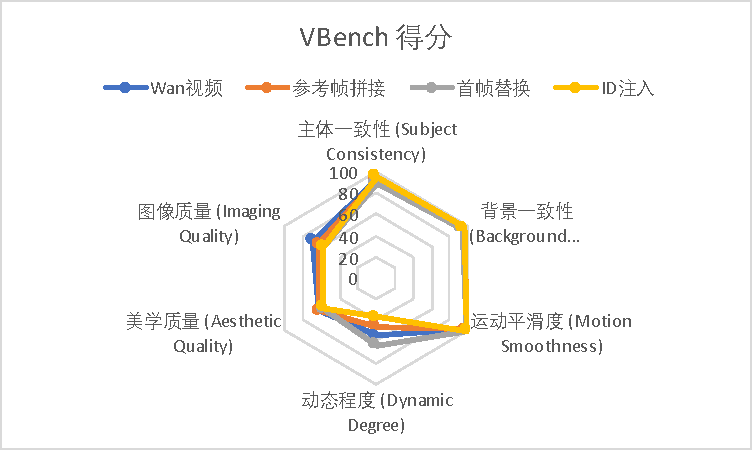
\includegraphics[width=0.8\textwidth]{final/Vbench.pdf}
    \caption{\textbf{VBench得分情况}}
    \label{fig:vbench}
\end{figure}

\subsection{高分辨率参考图视频生成方法效果评估} %[TODO]
为了验证所采用的基于流匹配的高效生成方法在推理速度上的优势,本文将其与当前若干主流的视频生成模型在不同分辨率和帧数设置下的每步推理时间(秒/步)进行了比较。详细的对比数据如表\ref{tab:time_size}和簇状条形图\ref{fig:time_size}所示。
\begin{table}[htbp]
    \centering
    \caption{不同模型参数量及在不同分辨率和帧数下的推理时间(秒/步)对比}
    \resizebox{1\linewidth}{!}{
    \renewcommand{\arraystretch}{1.2}
    \begin{tabular}{p{2.5cm} p{1.5cm} ccccccc}
    \toprule
    \multirow{2}{*}{\textbf{模型}} & \multirow{2}{*}{\textbf{参数量}} & \multicolumn{7}{c}{\textbf{推理时间 (秒/步)}} \\
    \cmidrule(lr){3-9}
     &  & \textbf{49 帧@720p} & \textbf{81 帧@720p} & \textbf{49 帧@1080p} & \textbf{81 帧@1080p} & \textbf{121 帧@1080p} & \textbf{49 帧@2k} & \textbf{81 帧@2k} \\
    \midrule
    CogvideoX\cite{yang2024cogvideox} & 2B & 4.27 & 9.74 & 32.13 & 79.64 & 171.49 & 95.05 & 248.76 \\
    CogvideoX\cite{yang2024cogvideox} & 5B & 11.12 & 24.47 & 76.60 & 188.29 & OOM & 225.8 & OOM  \\
    Hunyuan\cite{kong2024hunyuanvideo} & 13B & 11.43 & 29.14 & 98.54 & 258.95 & 552.12 & 326.96 & OOM\\ 
    Wanx Video\cite{wan2025} & 14B & 19.78 & 41.03 & 121.17 & 285.82 & OOM & 341.43 & OOM \\ \midrule
    \textbf{Ours} & 1B & 3.09 & 4.06 & 12.35 & 19.77 & 34.76 & 21.12 & 26.47 \\
    \bottomrule
    \end{tabular}
    }
    \label{tab:time_size}
\end{table}
\begin{figure}[htbp]
    \centering
    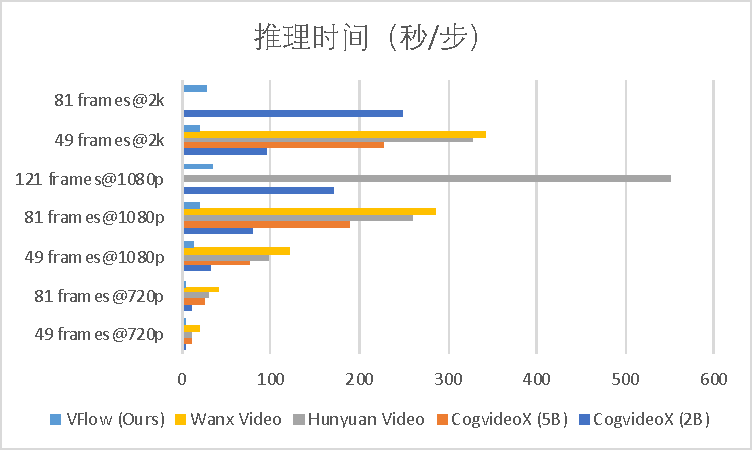
\includegraphics[width=0.8\textwidth]{final/Infer_time_compare.pdf}
    \caption{\textbf{不同模型在不同分辨率和帧数下的推理时间及其模型参数},其中推理时间本文使用推理每步的时长来衡量,单位为秒/步。
    }
    \label{fig:time_size}
\end{figure}
如表\ref{tab:time_size}和图\ref{fig:time_size}所示,本文比较了本文采用的1B参数量模型与其他参数规模更大(2B至14B)的主流模型(CogvideoX、Hunyuan Video、Wanx Video)的推理效率。

可以发现对于参数量为2B的CogvideoX模型,在生成49帧720p分辨率视频时,每步推理时间为4.27秒;当提升至81帧2K分辨率时,时间增加至248.76秒。更大参数量(5B)的CogvideoX模型在各配置下的推理时间均显著增加,并在处理121帧1080p及更高要求的任务时出现显存不足(OOM)的情况。
而对于Hunyuan Video (13B) 和 Wanx Video (14B) 这种更大参数量的模型,虽然可能在生成质量上具有优势,但在推理时间上表现出更高的开销。例如,Hunyuan Video在121帧1080p时耗时552.12秒/步,Wanx Video在类似配置下也面临OOM问题或极高的推理时长。

与之形成鲜明对比的是,本文采用的1B参数量轻量级模型,在所有测试配置下的每步推理时间均表现出显著优势。特别是在49帧720p(3.09秒/步)和81帧720p(4.06秒/步)分辨率下,其推理时间远低于其他模型。在更高分辨率和帧数的挑战下,例如49帧2K(21.12秒/步)和81帧2K(26.47秒/步),本方法依然保持了较高的推理效率,并且能够成功运行而未出现OOM,这对于资源受限的应用场景尤为重要。
\begin{table}[!t]
\centering
\caption{本文方法和其他超分方法在图片质量和视频质量方面数值对比}
% \begin{adjustbox}{width=\hsize}
\small
\begin{tabular}{lcccccc}
\toprule
& \multicolumn{3}{c}{\textbf{图片质量}} & \multicolumn{3}{c}{\textbf{视频质量 \cite{dover}}} \\
\cmidrule(lr){2-4} \cmidrule(lr){5-7} 
\textbf{方法} & \textbf{MUSIQ\cite{ke2021musiq}$\uparrow$} & 
\textbf{MANIQ\cite{maniqa}$\uparrow$} &
\textbf{NIQE\cite{niqe}$\downarrow$} &  
\textbf{Tech.$\uparrow$} & \textbf{Aesth.$\uparrow$} \\
\midrule
RealBasicVSR\cite{RealBasicVSR} &53.85 &0.269&5.257 &99.86& 8.75 \\
Upscale-a-Video\cite{zhou2024upscaleavideo}&40.40 &0.237 &6.604 & 99.22& 7.00\\
VEhancer\cite{he2024venhancer}&45.39 &0.258 &5.894&99.64&9.75\\
\bottomrule
本文的方法&41.33 &0.233 & 5.750&99.55&9.16 \\
\end{tabular}
% \end{adjustbox}
% \vspace{-0.1in}
% \vspace{-0.1in}
\label{tab:vsr_compare}
\end{table}
该表格和图表的对比清晰地展示了不同模型在推理效率上的巨大差异,有力地证明了本文采用的基于流匹配的轻量级模型在保证生成能力的同时,能够在高分辨率视频生成任务中提供更高效的推理表现。
\begin{figure}[h]
    \centering
    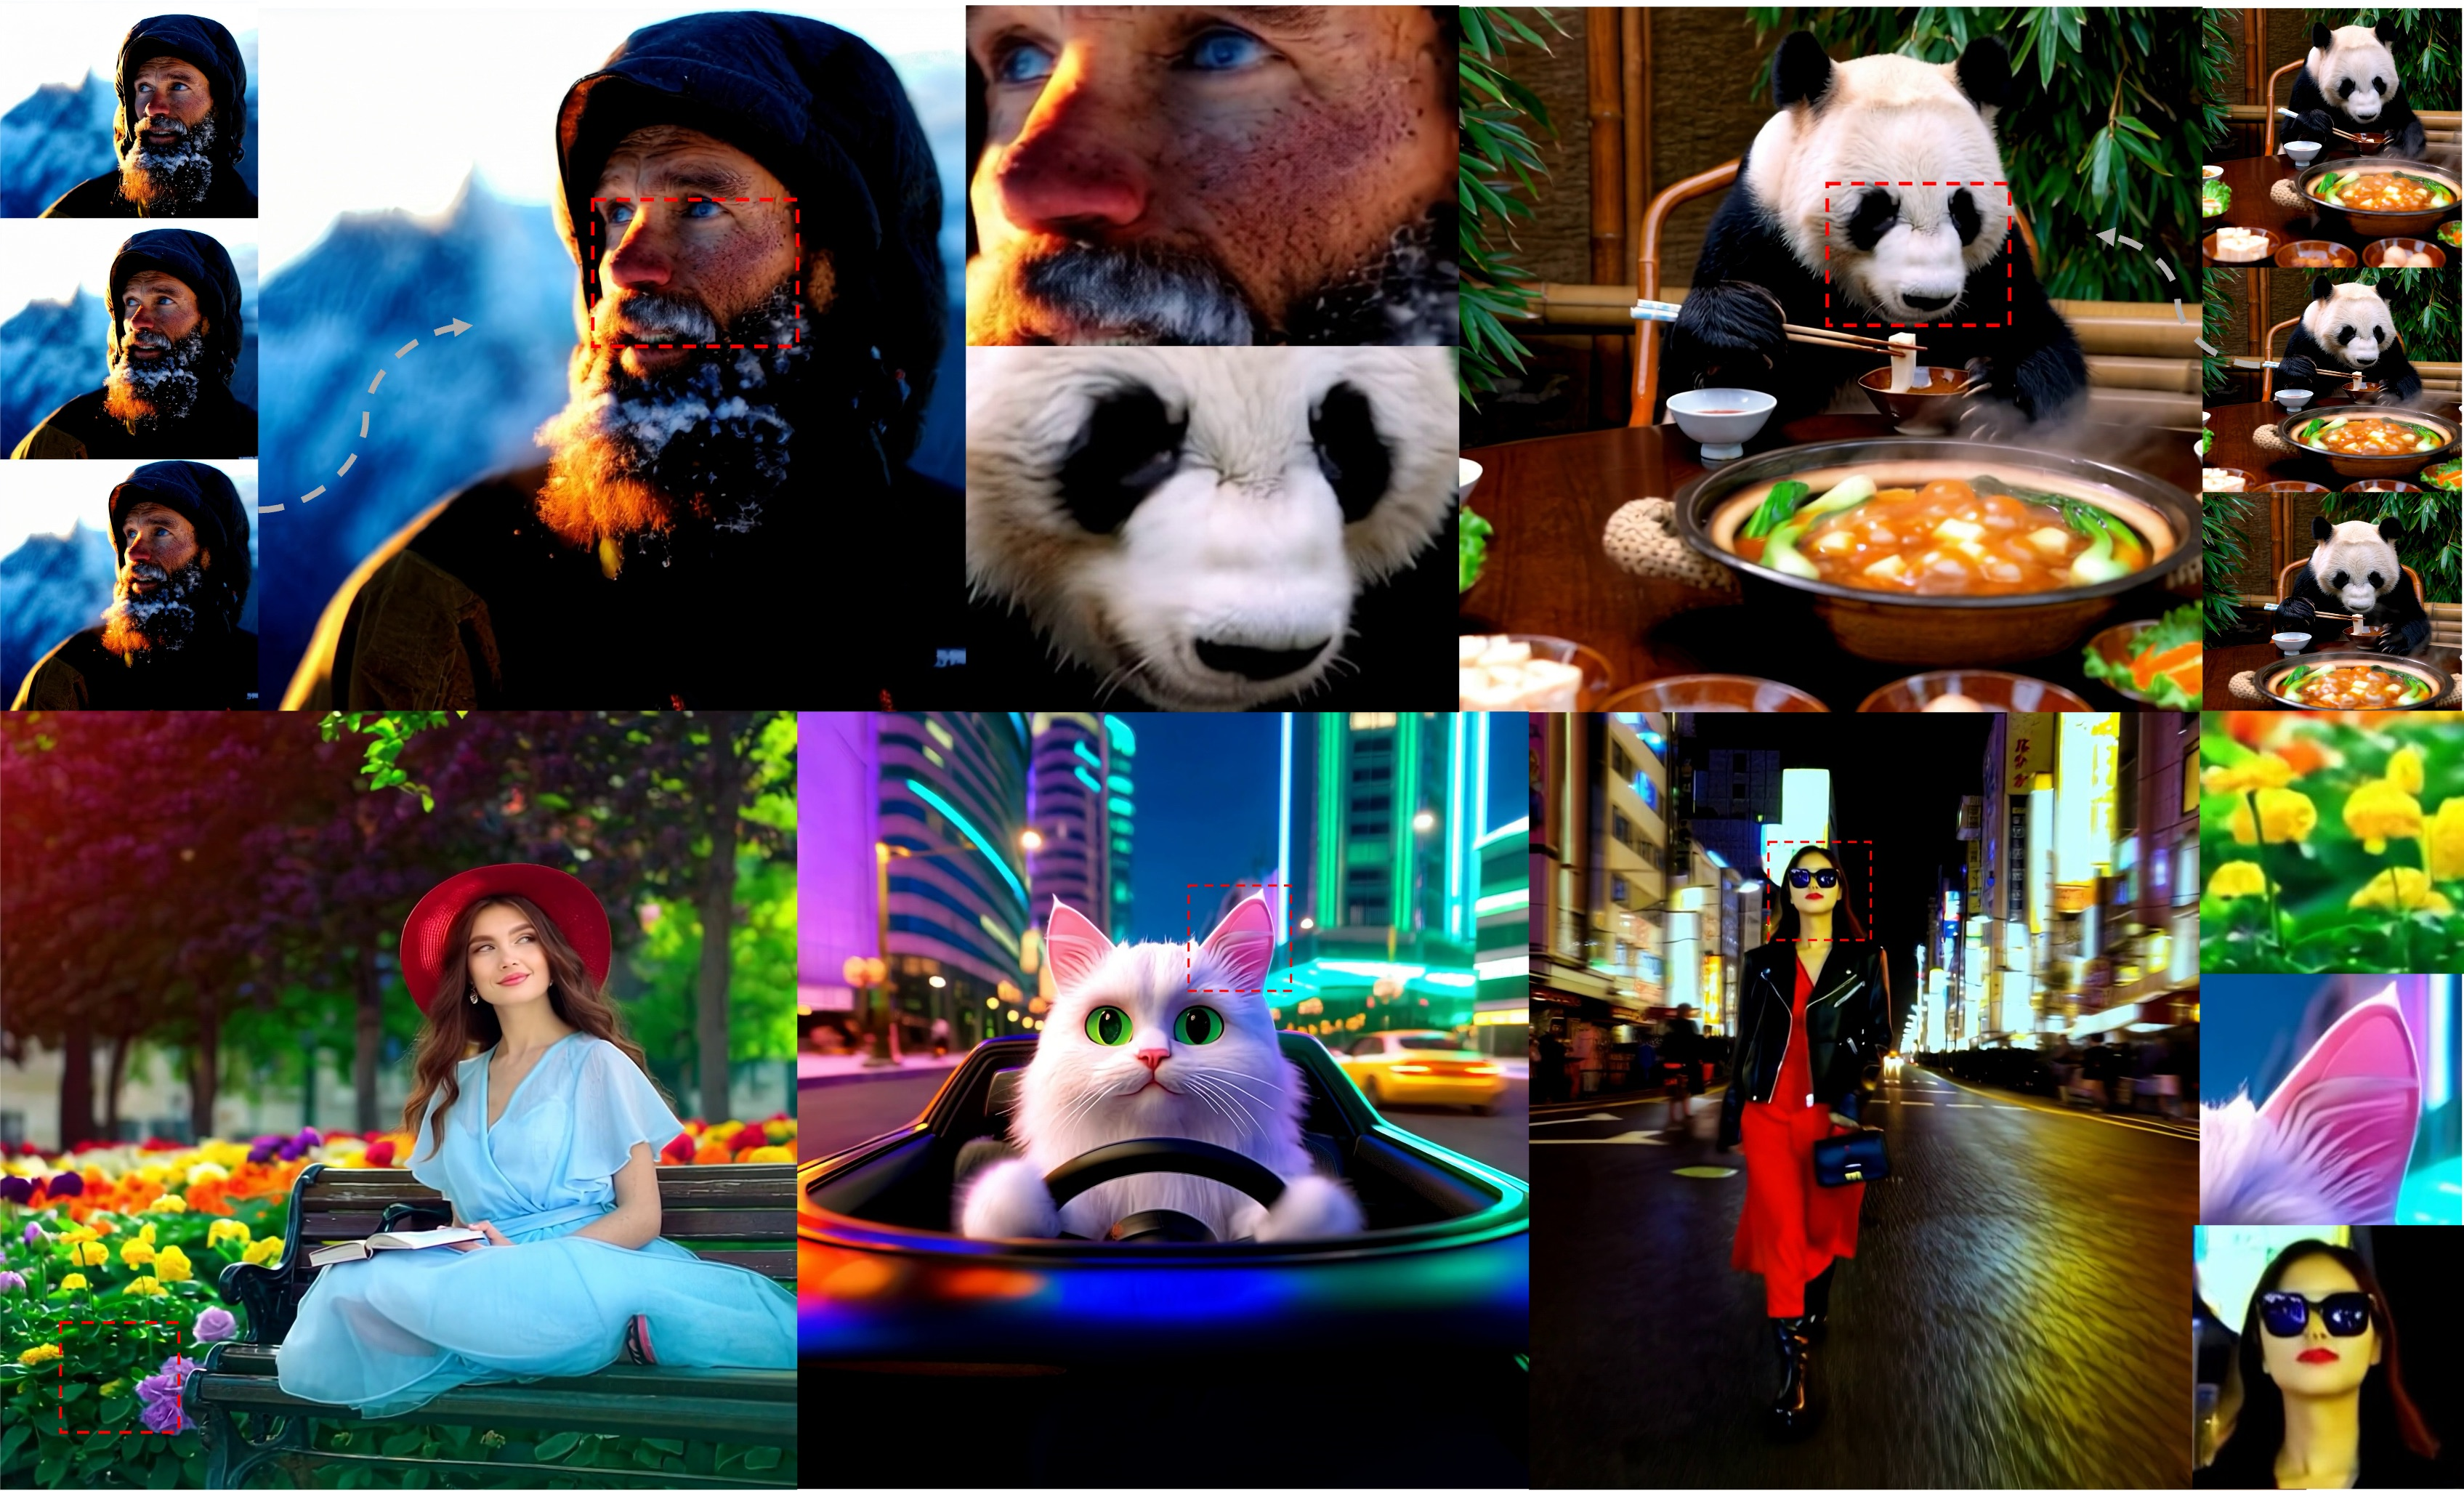
\includegraphics[width=0.8\textwidth]{final/hqvideo.pdf}
    \caption{\textbf{高分辨率视频生成结果展示}:示例了采用本文提出的高效方法生成的720p或更高分辨率的视频帧。}
    \label{hqvideo}
\end{figure}
通过采用上述高效的流匹配生成方法,本文成功生成了一系列高分辨率视频。图\ref{hqvideo}展示了部分生成结果的样例。这些结果表明,即便在使用了参数量较小的模型和显著加速的推理流程下,所生成视频仍然能够保持较好的视觉质量、细节丰富度以及与参考图像内容的一致性。更多对比视频展示如图\ref{fig:vsr2}、\ref{fig:vsr3}和\ref{fig:vsrcompare}。

\begin{figure}[h]
    \centering
    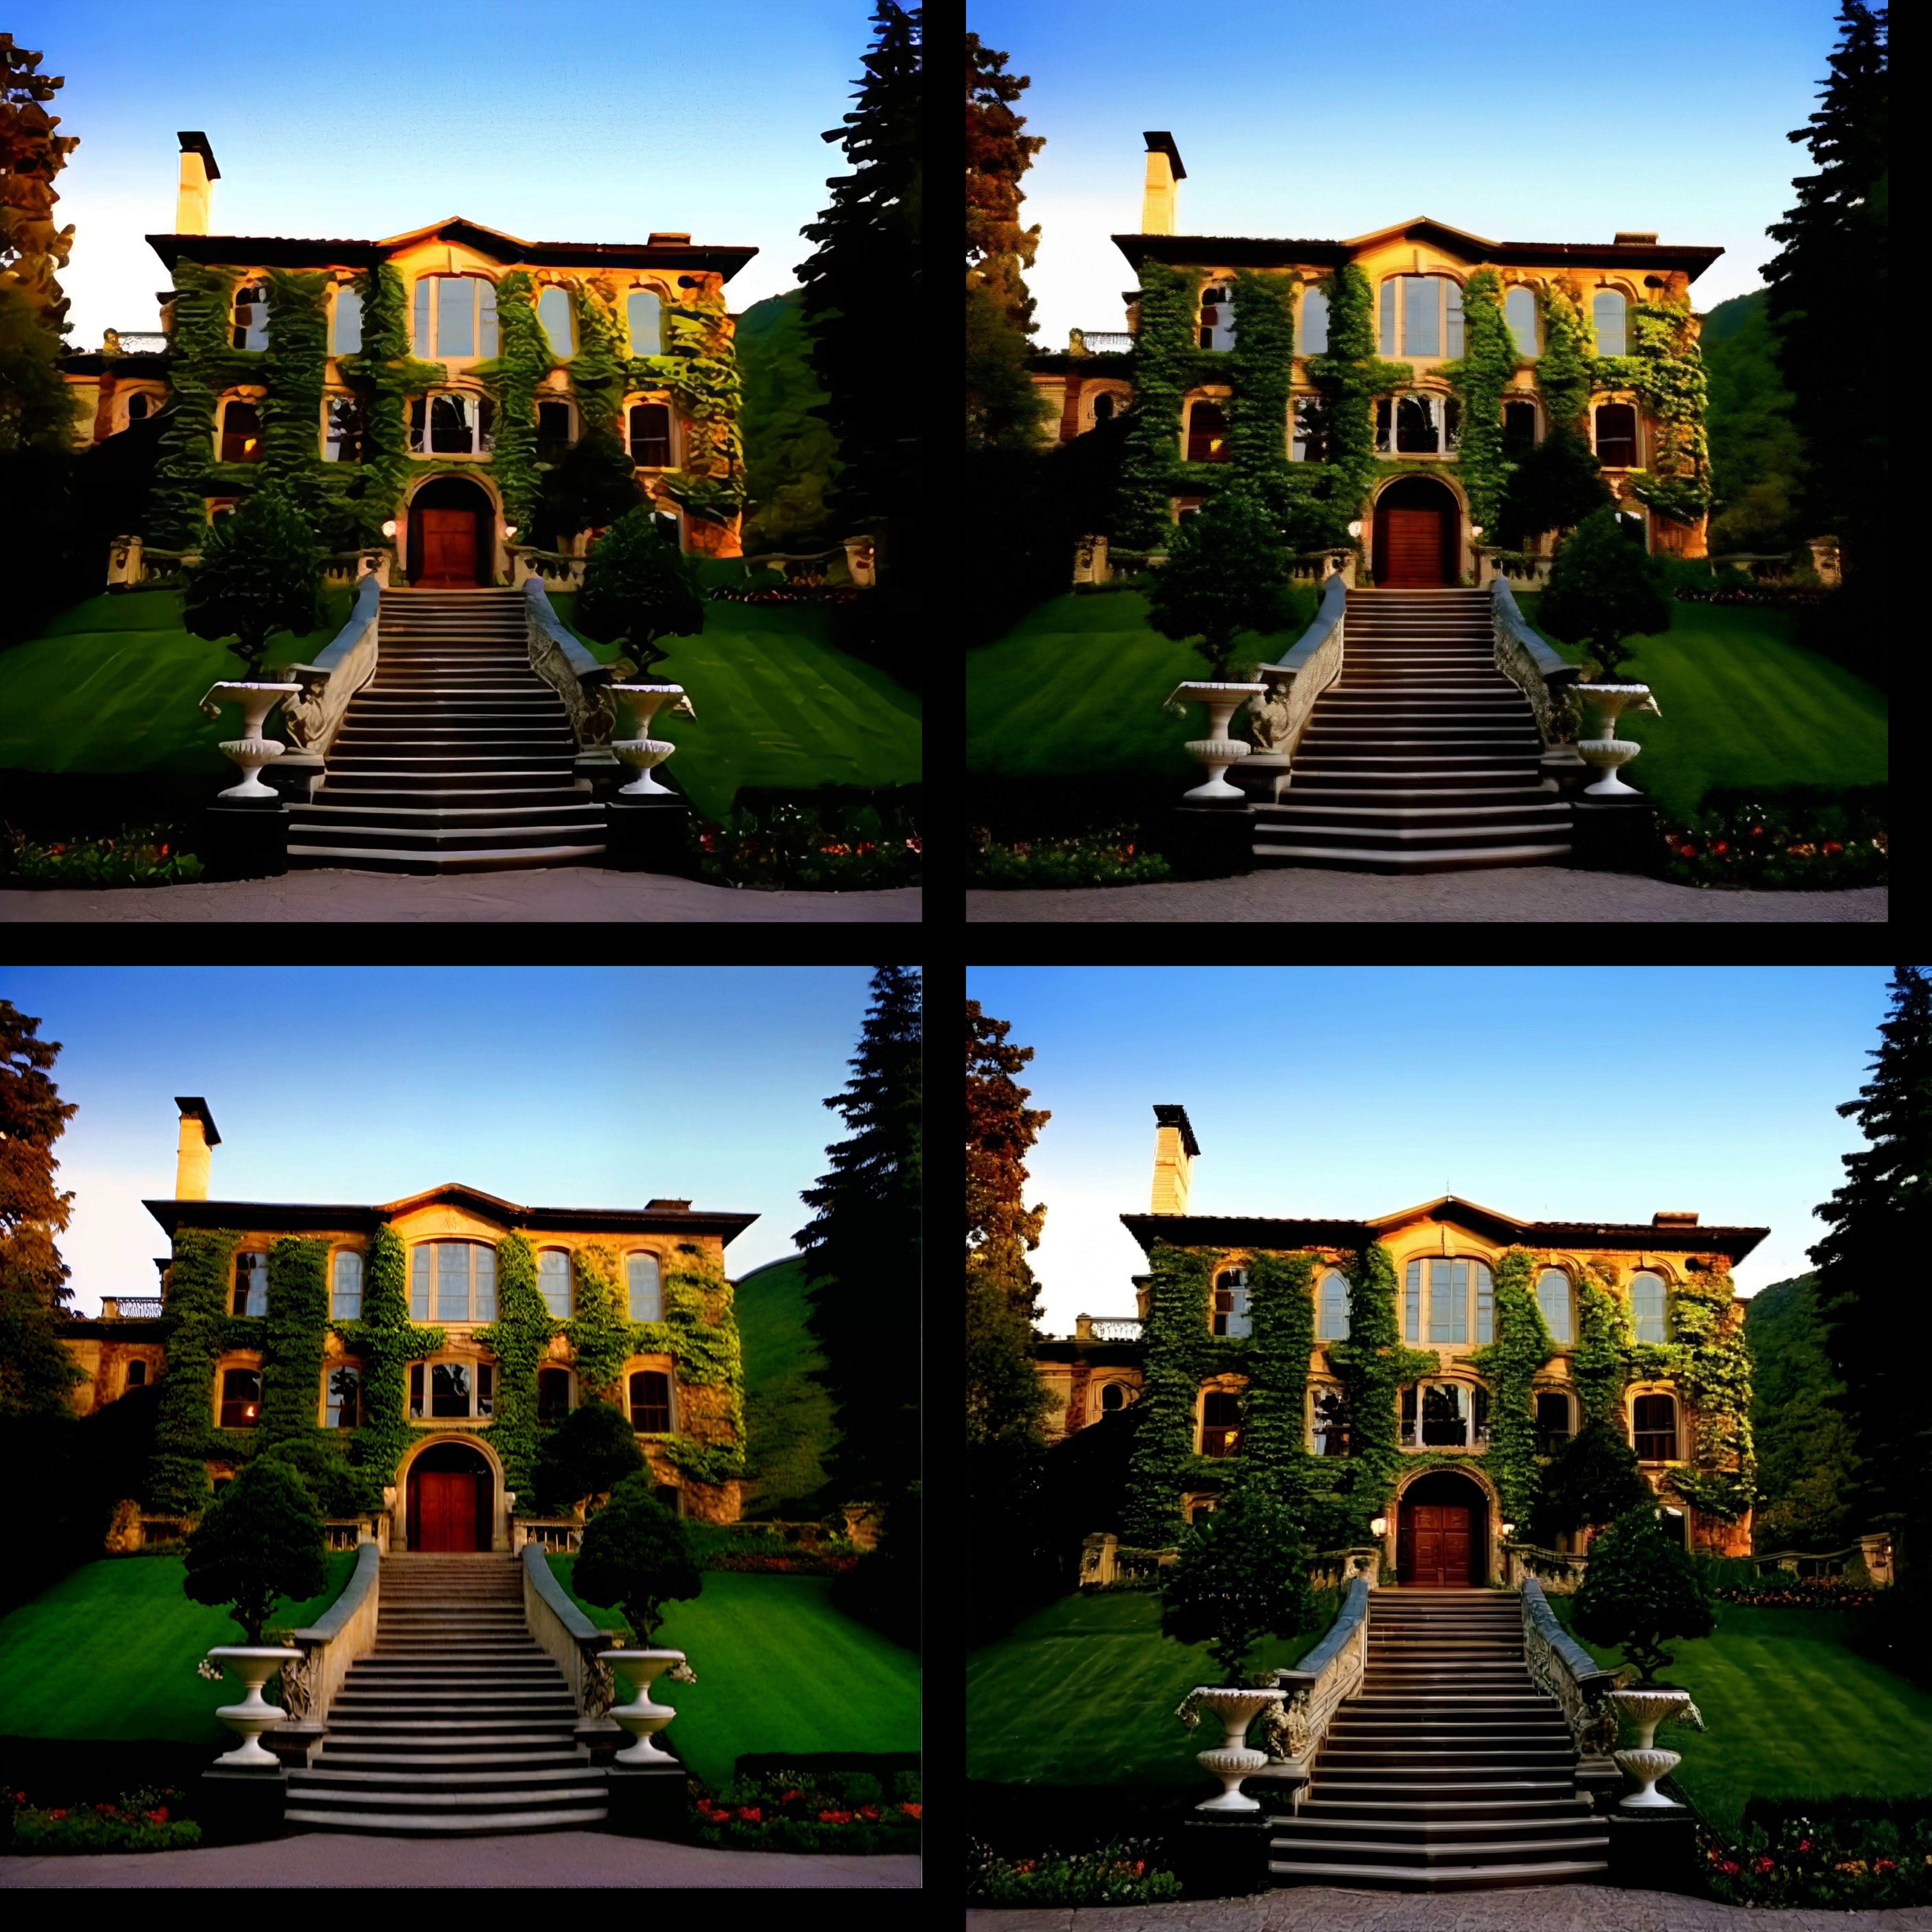
\includegraphics[width=0.7\textwidth]{final/VSRcompare.pdf}
    \caption{\textbf{其中左下角为通过线性变化得到的视频,左上角为RealBasicVSR方法超分的视频,右上角为Upscale-A-Video获得的视频,右下角为本文方法测试的数据。} 可以发现房屋的纹理细节,还是不合理地方的生成式修复都是本文的方法更占有}
    \label{fig:vsr2}
\end{figure}

\begin{figure}[h]
    \centering
    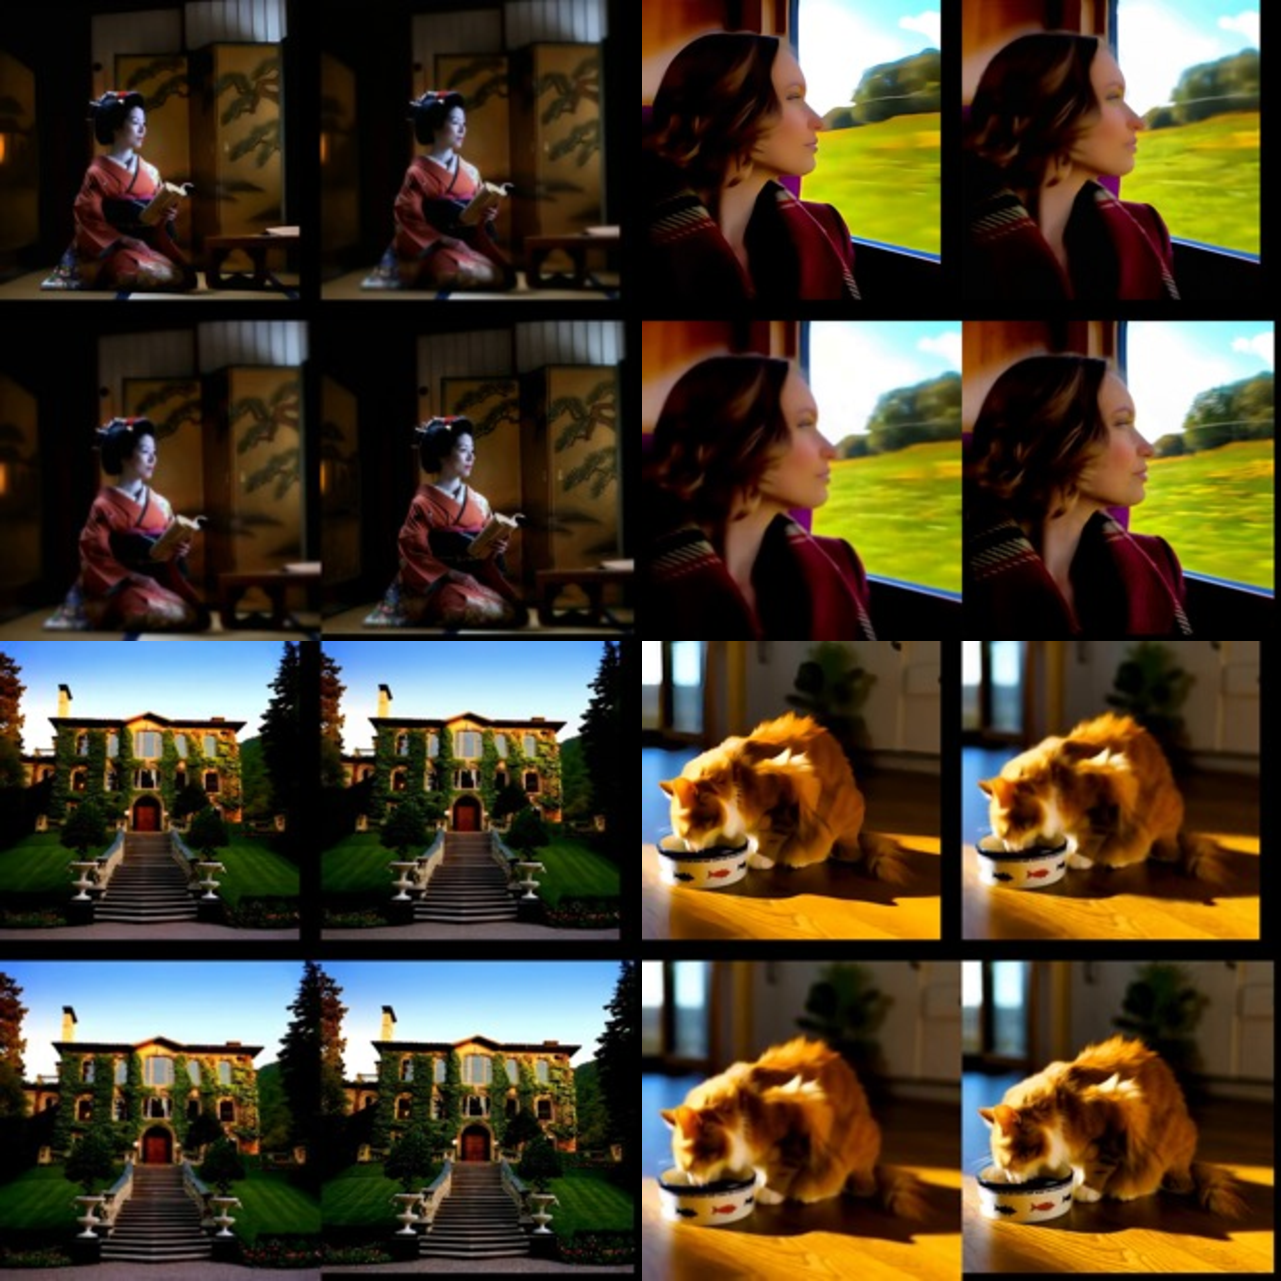
\includegraphics[width=0.7\textwidth]{final/VSR_compare_1.pdf}
    \caption{关于本文方法的更多例子。对于每个四方格,其中左下角为通过线性变化得到的视频,左上角为RealBasicVSR方法超分的视频,右上角为Upscale-A-Video获得的视频,右下角为本文方法测试的数据。 }
    \label{fig:vsr3}
\end{figure}

\begin{figure}[h]
    \centering
    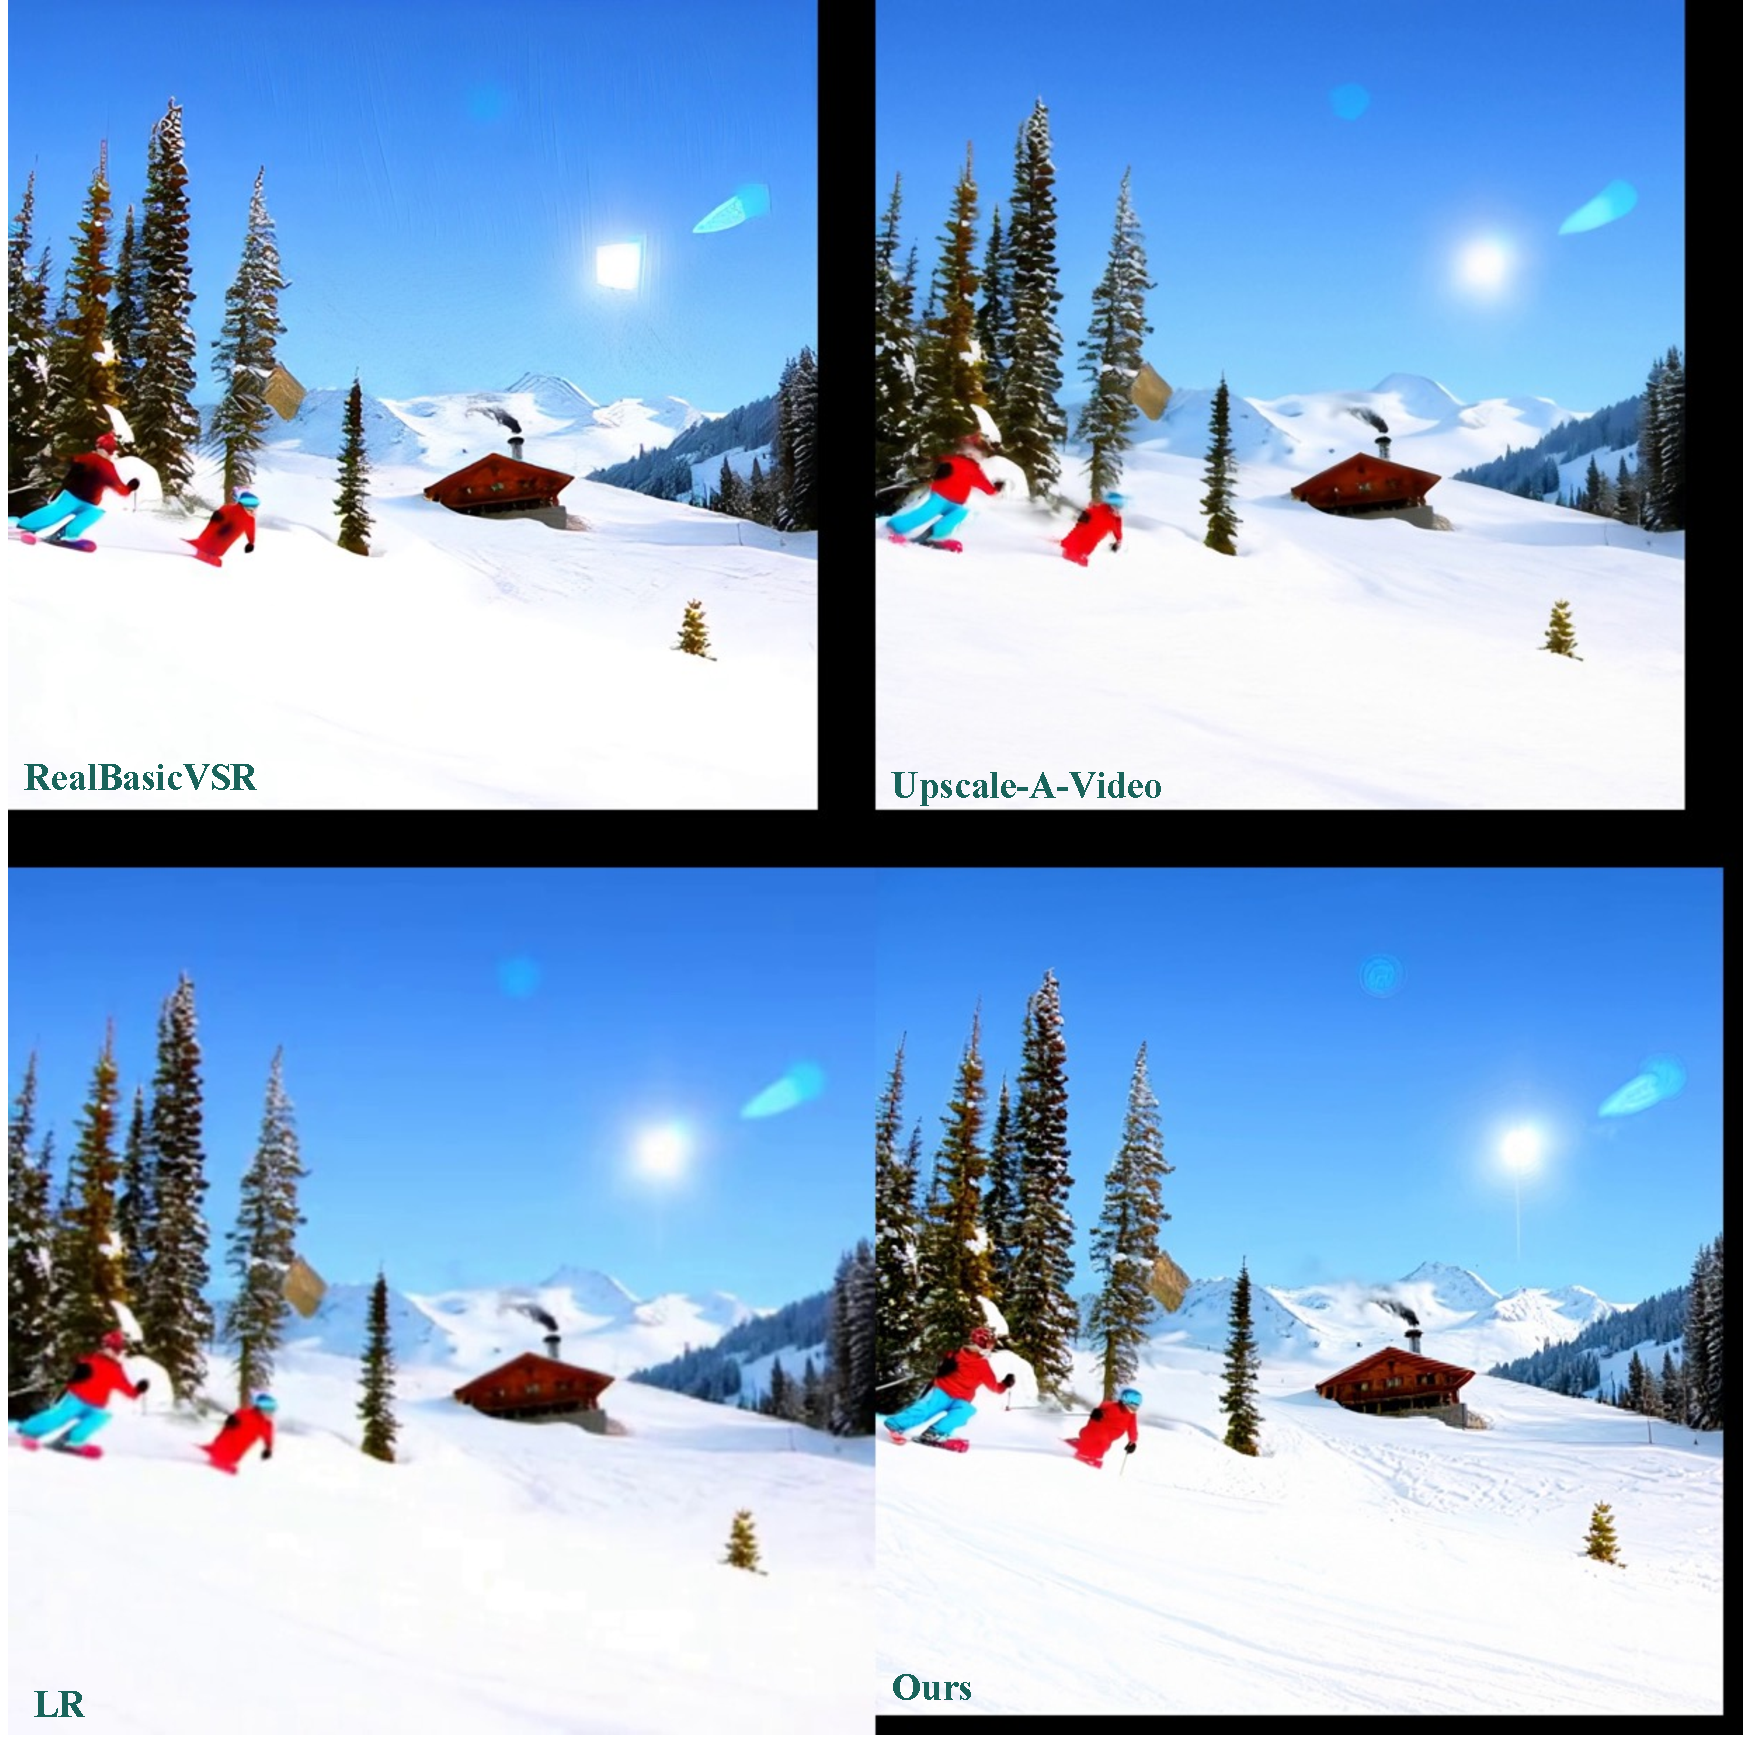
\includegraphics[width=0.7\textwidth]{final/vsr_compare.pdf}
    \caption{\textbf{其中左下角为通过线性变化得到的视频,左上角为RealBasicVSR方法超分的视频,右上角为Upscale-A-Video获得的视频,左下角为输入的低分辨率视频,右下角为本文方法测试的数据。}可以发现滑雪人的清晰度是本文方法最优秀。}
    \label{fig:vsr1}
\end{figure}


本文将前面章节获得的低分辨率视频通过线性变换到目标分辨率(如,1080p, 2K) 这时候由于并没有新的像素产生,所以得到的视频对应为低分辨率视频,如图\ref{fig:vsr2}的左下角。可以明显看出本文方法的生成式修复能力最佳。为直观评估本文方法的性能,本文将其与当前几种先进的VSR方法进行了视觉效果对比,包括RealBasicVSR\cite{RealBasicVSR}、Upscale-a-Video\cite{zhou2024upscaleavideo}以及VEhancer\cite{he2024venhancer}。对比基准(baseline)为通过标准线性插值方法从低分辨率视频直接放大得到的视频帧。

如图\ref{fig:vsr2}、图\ref{fig:vsr3}和图\ref{fig:vsr1}所示,每组对比均包含四个子图:左下角为线性插值放大的低分辨率视频帧,作为参照;左上角为RealBasicVSR方法的超分结果;右上角为Upscale-A-Video方法的超分结果;右下角则为本文方法本文方法的处理结果。


通过对图\ref{fig:vsr2}、图\ref{fig:vsr3}和图\ref{fig:vsr1}中各对比案例的细致观察,可以发现本文方法本文方法在生成式修复能力方面展现出显著的优越性。尽管一些对比方法在特定指标上可能表现良好,但其实际视觉效果可能存在不足。例如,RealBasicVSR\cite{RealBasicVSR}方法生成的视频帧有时会呈现色彩过渡不够平滑、大面积区域色彩单一的问题,导致画面可能因此缺乏丰富的细节层次和细腻的纹理特征。

相比之下,VEhancer\cite{he2024venhancer}虽然能够有效加强图像的既有细节,但在处理输入图像中本身就因严重模糊而信息大量丢失的区域(例如人物的眉眼部分)时,其“从无到有”的生成能力则相对有限,难以凭空创造出清晰、自然的生物特征。而本文提出的本文方法方法,则在这些方面表现出更强的综合能力。它不仅能够有效加强和复刻材质纹理,例如在图\ref{fig:vsr2}中清晰地再现出墙壁上石头的颗粒质感;更重要的是,如图\ref{fig:vsr3}中的部分人脸细节修复案例所示,本文方法能够凭借其从大规模数据中学习到的强大先验知识,对人物模糊的面部进行智能地补全与细致复原,生成出结构合理、清晰可辨的眉毛、眼睛和嘴部等关键特征。这种优秀的生成式修复能力使得本文方法在提升视觉真实感和细节丰富度方面具有明显优势。


除了定性视觉比较外,本文还使用一系列公认的图像及视频质量评估指标对本文方法及其他SOTA VSR方法进行了严格的定量分析。详细对比结果如表\ref{tab:vsr_compare}所示。
从表\ref{tab:vsr_compare}的定量结果中可以看出,在帧级质量评估方面,本文方法取得了MUSIQ 41.33分,MANIQ 0.233分,以及NIQE 5.750分的成绩。虽然这些单帧的无参考质量评估指标并非在所有对比方法中均达到最优(例如RealBasicVSR在这些指标上数值领先),但值得强调的是,正如前文定性分析所指出的,单纯依赖像素级或统计学上的客观指标有时难以完全捕捉和反映生成内容的实际视觉感受、细节恢复的精妙程度以及生成式修复的合理性。某些情况下,较高的客观指标得分可能伴随着如纹理过度平滑或不自然的人工痕迹等视觉缺陷。

在更能体现视频综合观感的DOVER视频质量评价体系中,本文方法在技术质量(Tech.)方面取得了99.55分,与VEhancer(99.64分)和RealBasicVSR(99.86分)等顶尖方法处于同一水平,这表明其生成的视频在基础的清晰度、运动连贯性、伪影抑制等方面均符合极高的技术标准。更为关键的是,在美学质量(Aesth.)方面,本文方法获得了9.16分,该项得分不仅显著优于RealBasicVSR(8.75分)和Upscale-a-Video(7.00分),并且接近表现最佳的VEhancer(9.75分)。这有力地证明了本文方法在生成视觉上更自然、细节更丰富、整体观感更令人愉悦的超分辨率视频方面具有强大的竞争力。因此,综合考量定量指标与实际视觉效果,尤其是在结合其优秀的生成式修复能力进行评估时,本文方法展现了作为一种先进VSR解决方案的巨大潜力。

值得注意的是,本文发现用于提升视频质量的模型训练成本相对较低,远低于实现其他功能性改进所需的资源开销。本文推测,这一现象可能归因于低分辨率视频作为条件输入降低了模型在学习过程中对视觉效果提升的难度。因此,在已有结构下,模型更容易专注于局部细节还原和视觉清晰度增强,而无需构建复杂的全局语义理解能力。\

\begin{figure}[H]
    \centering
    % 单独展示 Ours
    \begin{subfigure}[b]{0.9\textwidth}
        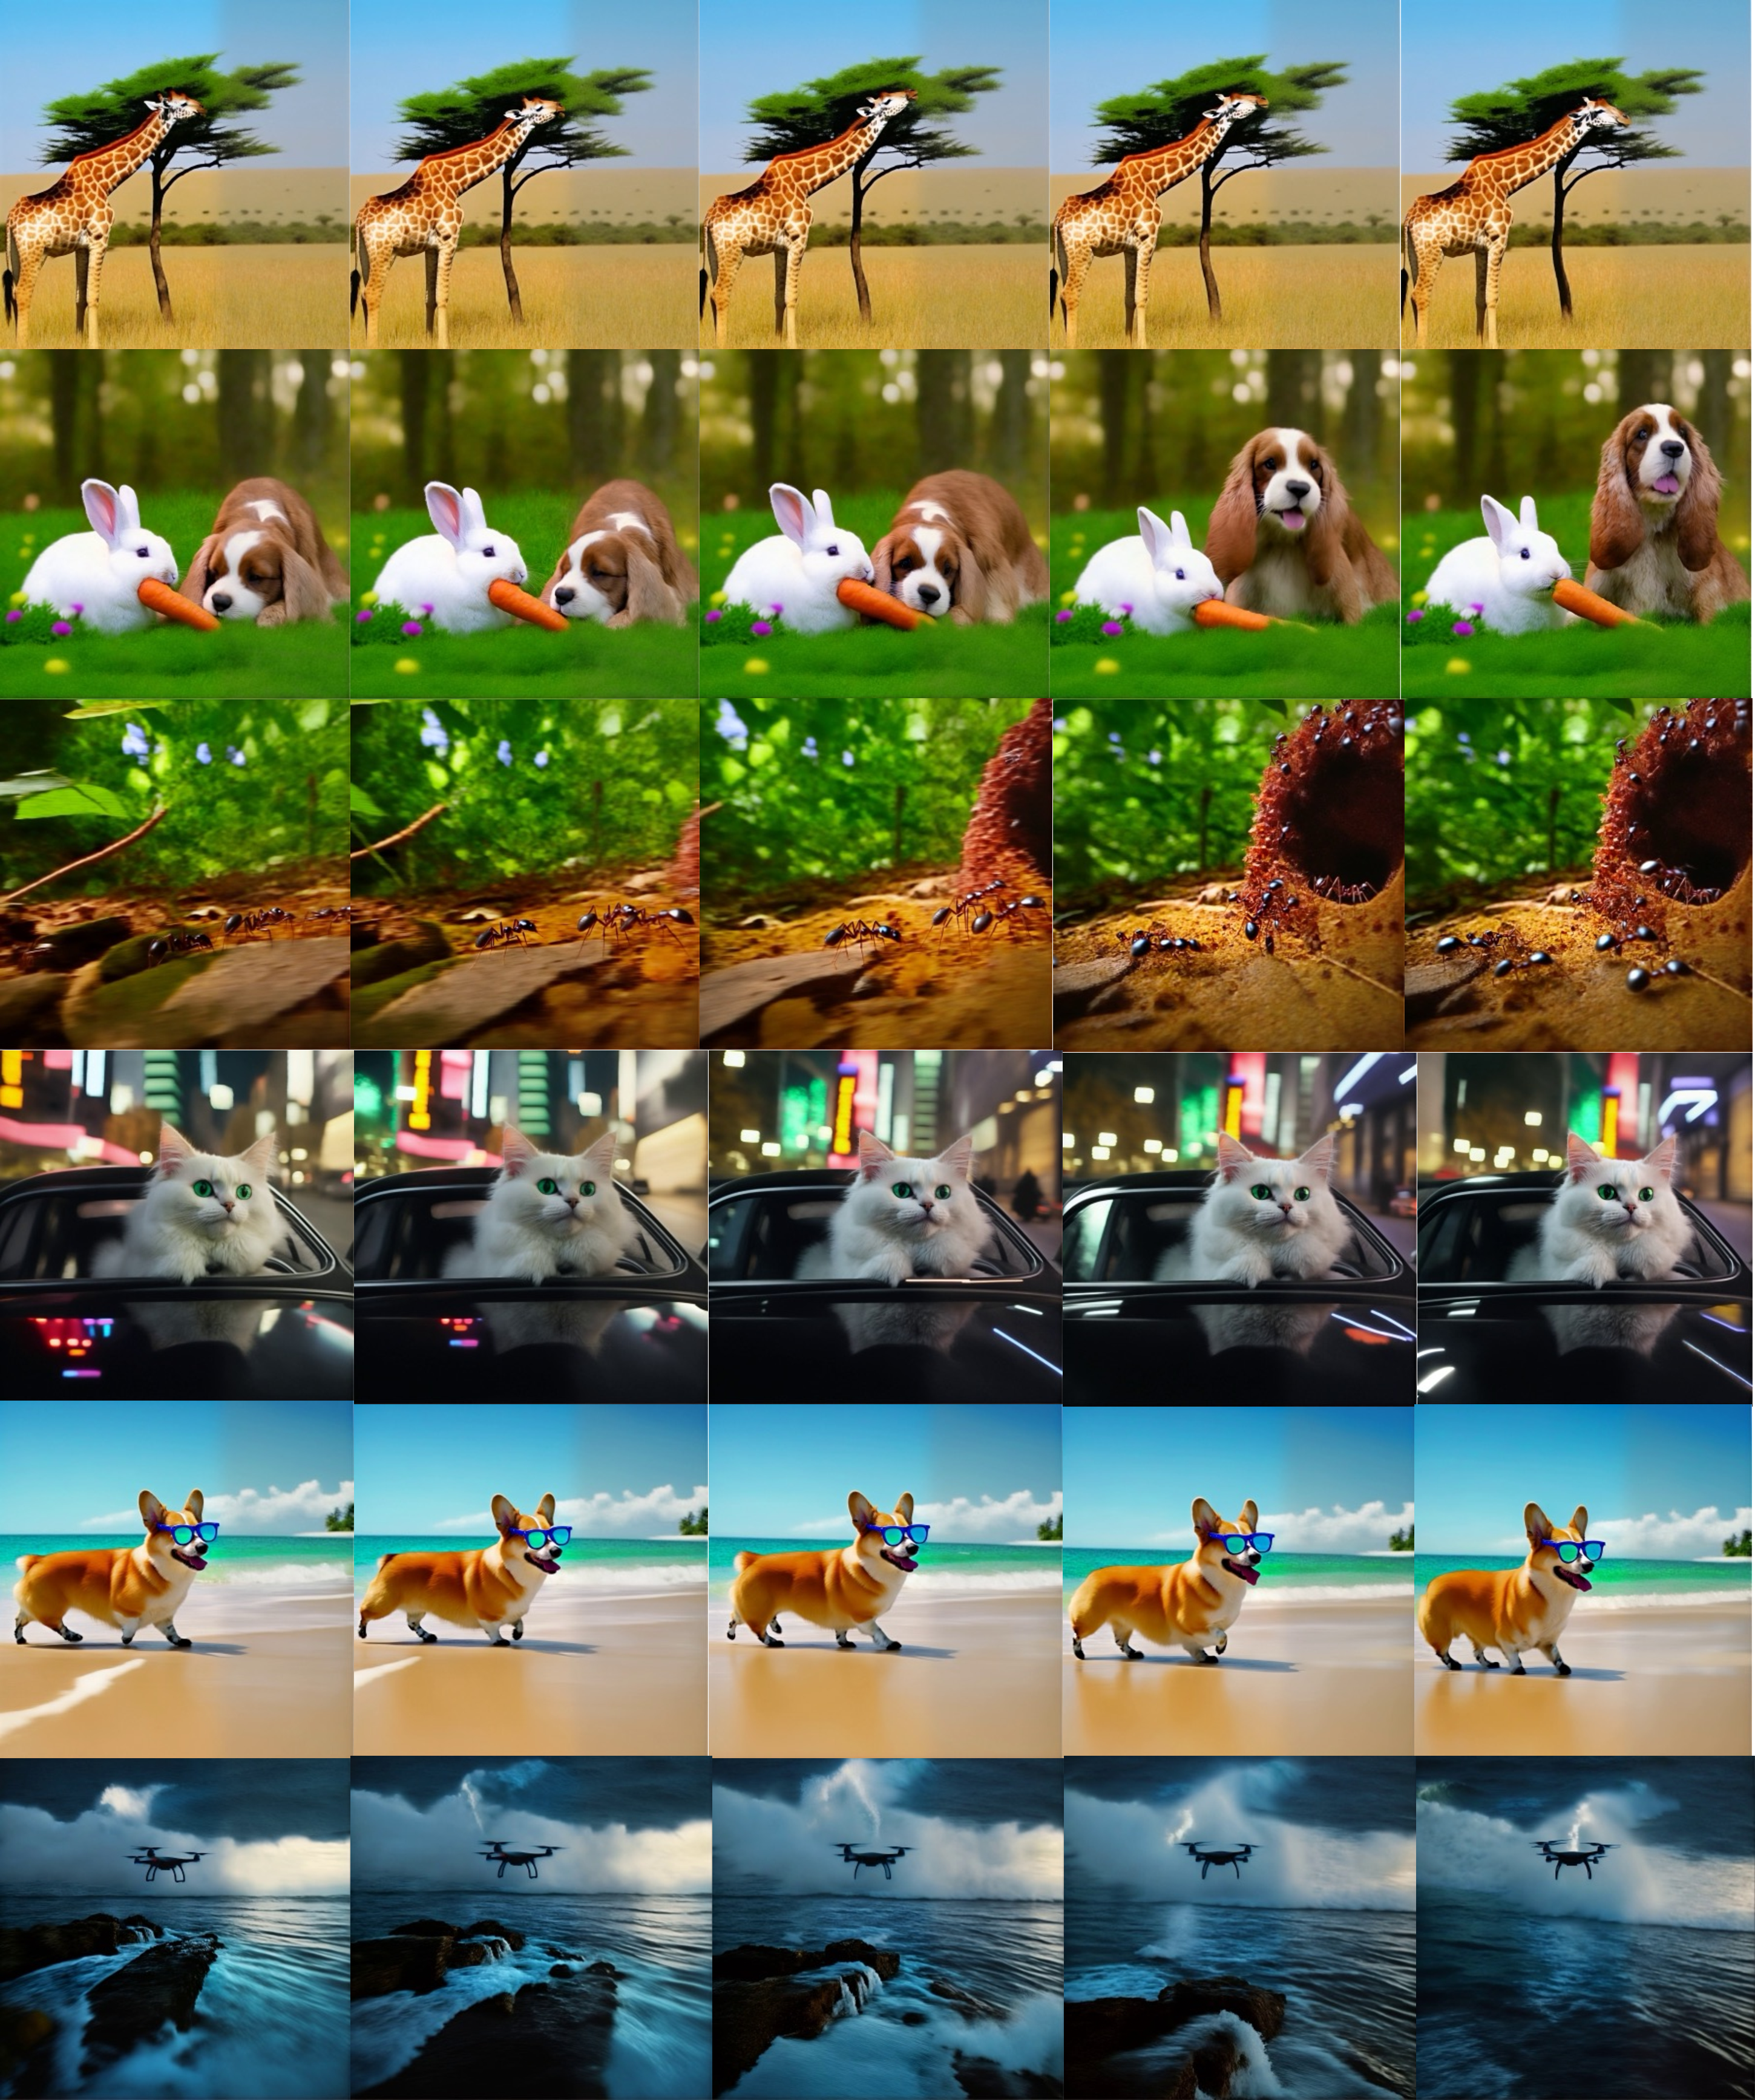
\includegraphics[width=\textwidth]{final/ours.pdf}
        \caption{我们的方法}
        \label{fig:ours}
    \end{subfigure}

    \vspace{0.5em} % 控制上下间距

    % 3个上下拼接展示
    \begin{subfigure}[b]{0.3\textwidth}
        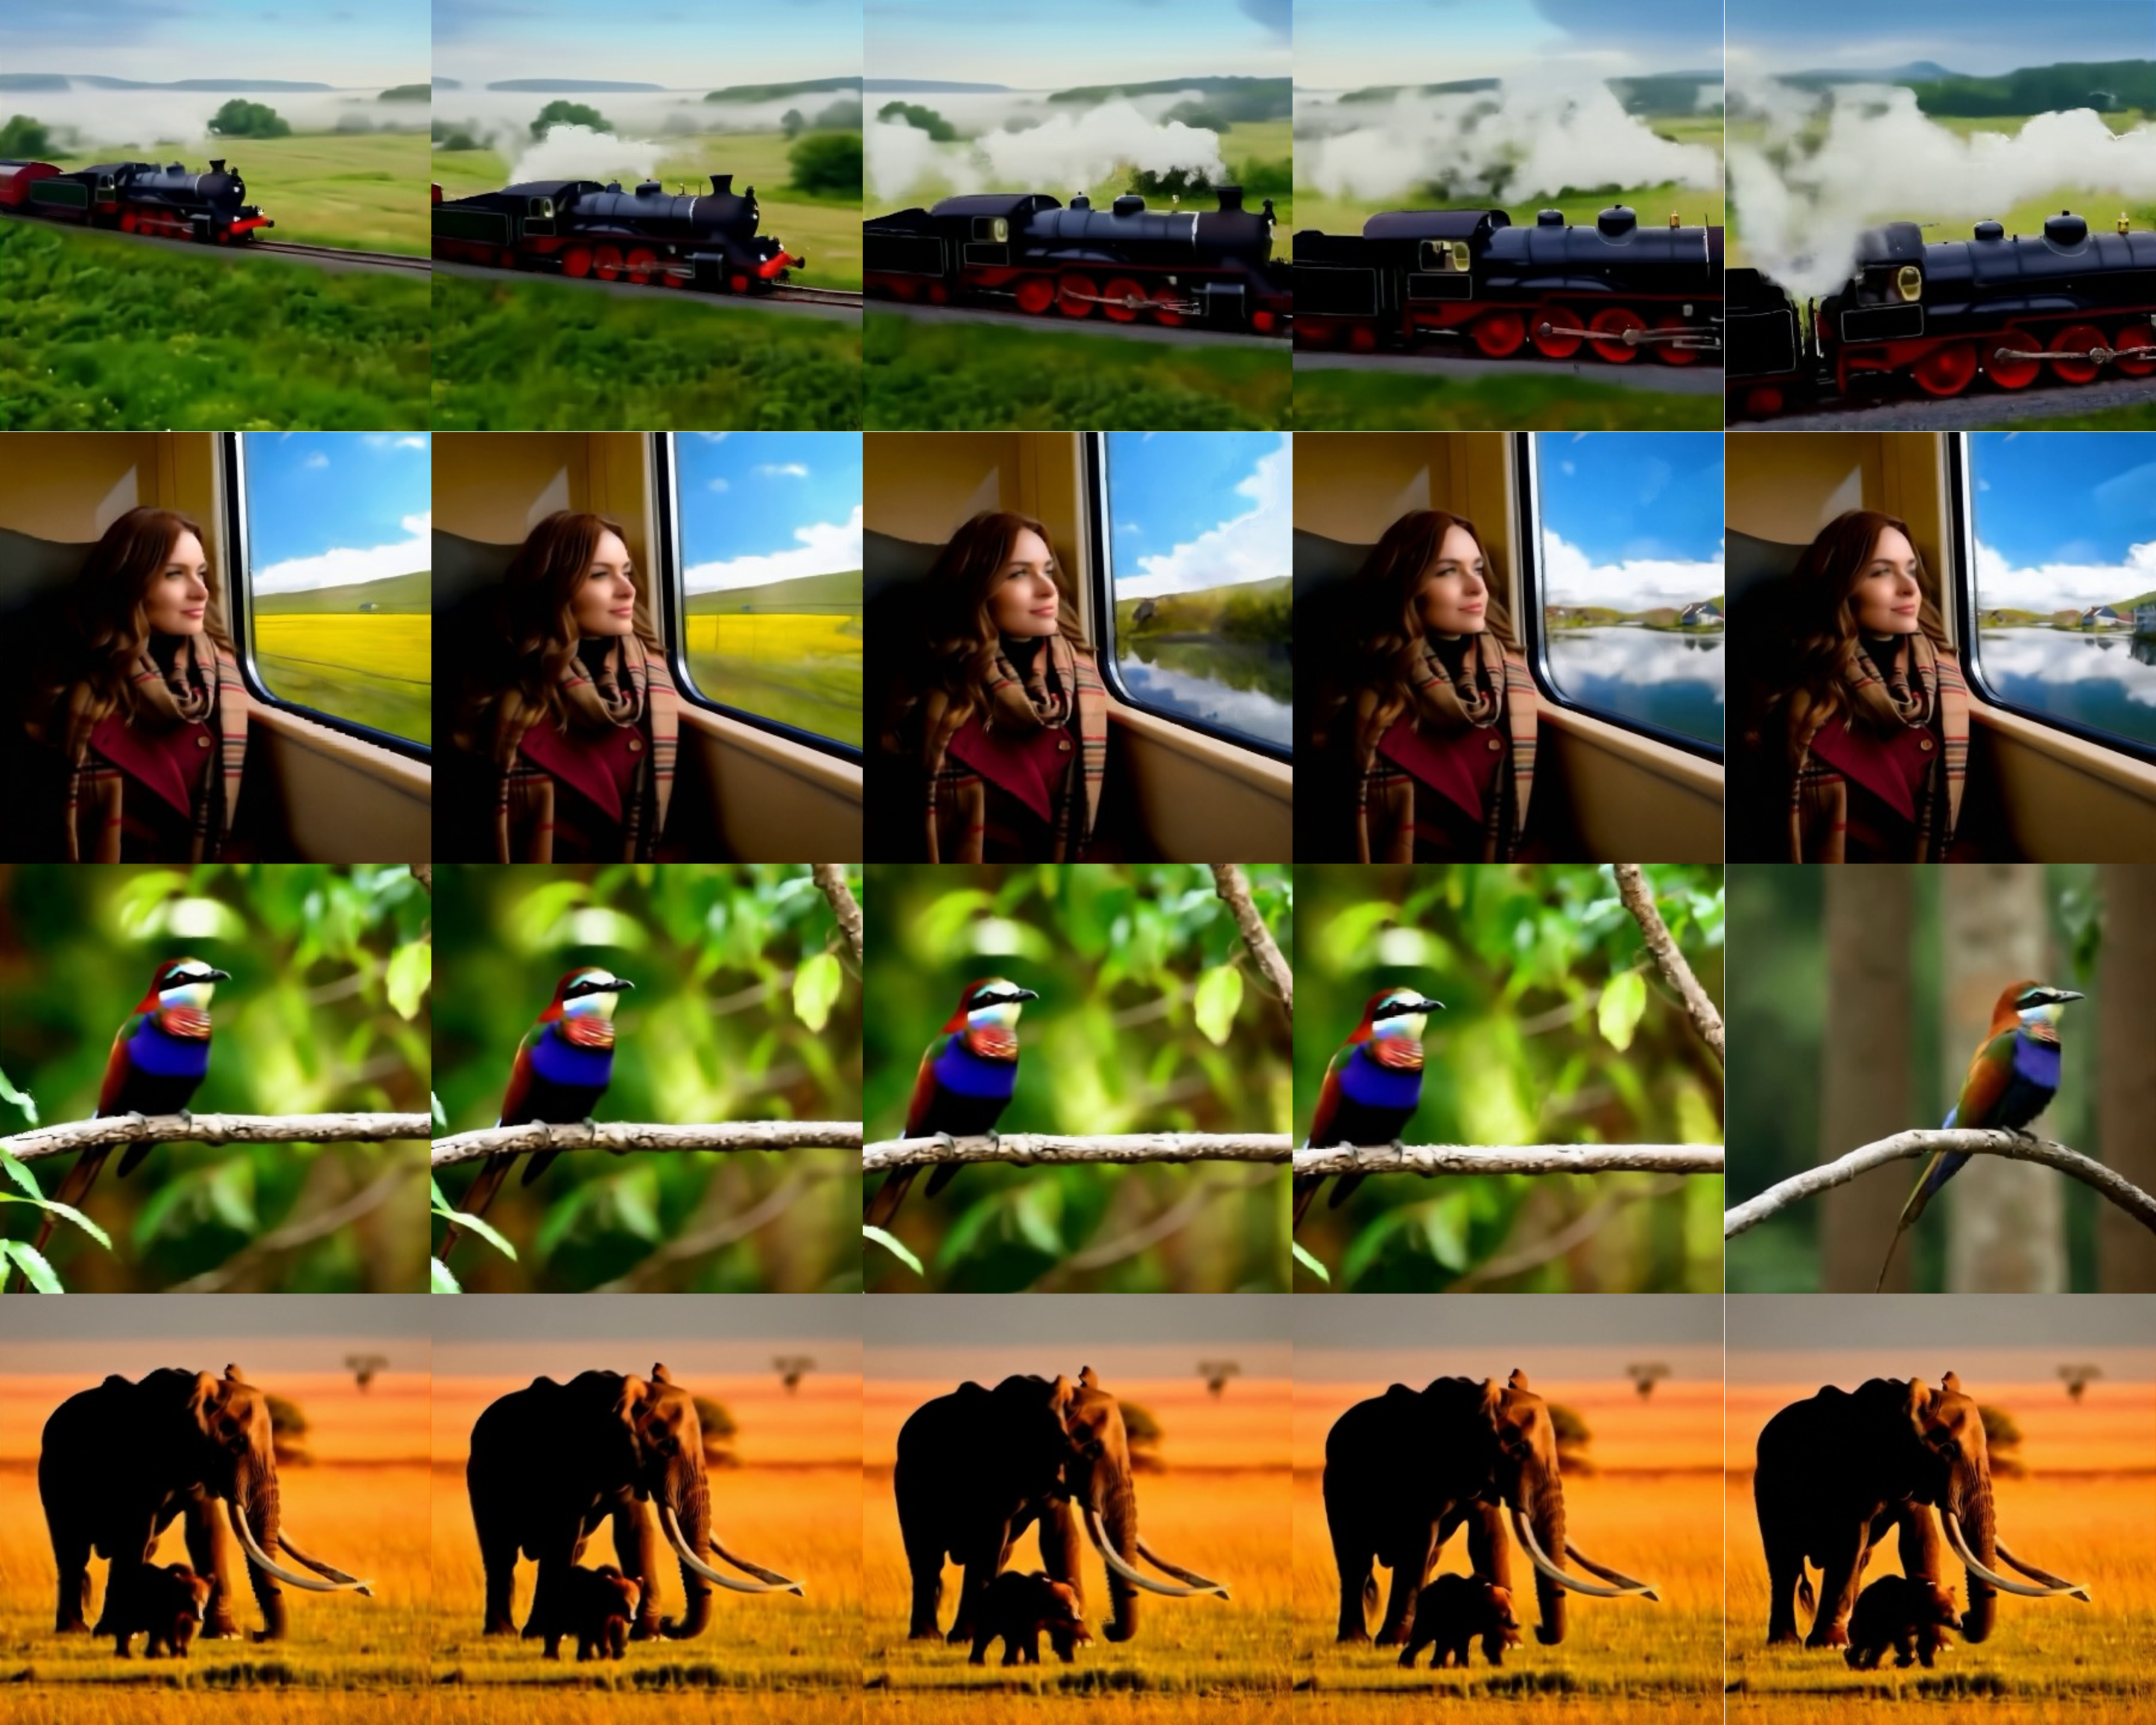
\includegraphics[width=\textwidth]{final/Upscale-A-Video.pdf}
        \caption{Upscale-A-Video方法}
        \label{fig:upscale}
    \end{subfigure}
    \hfill
    \begin{subfigure}[b]{0.3\textwidth}
        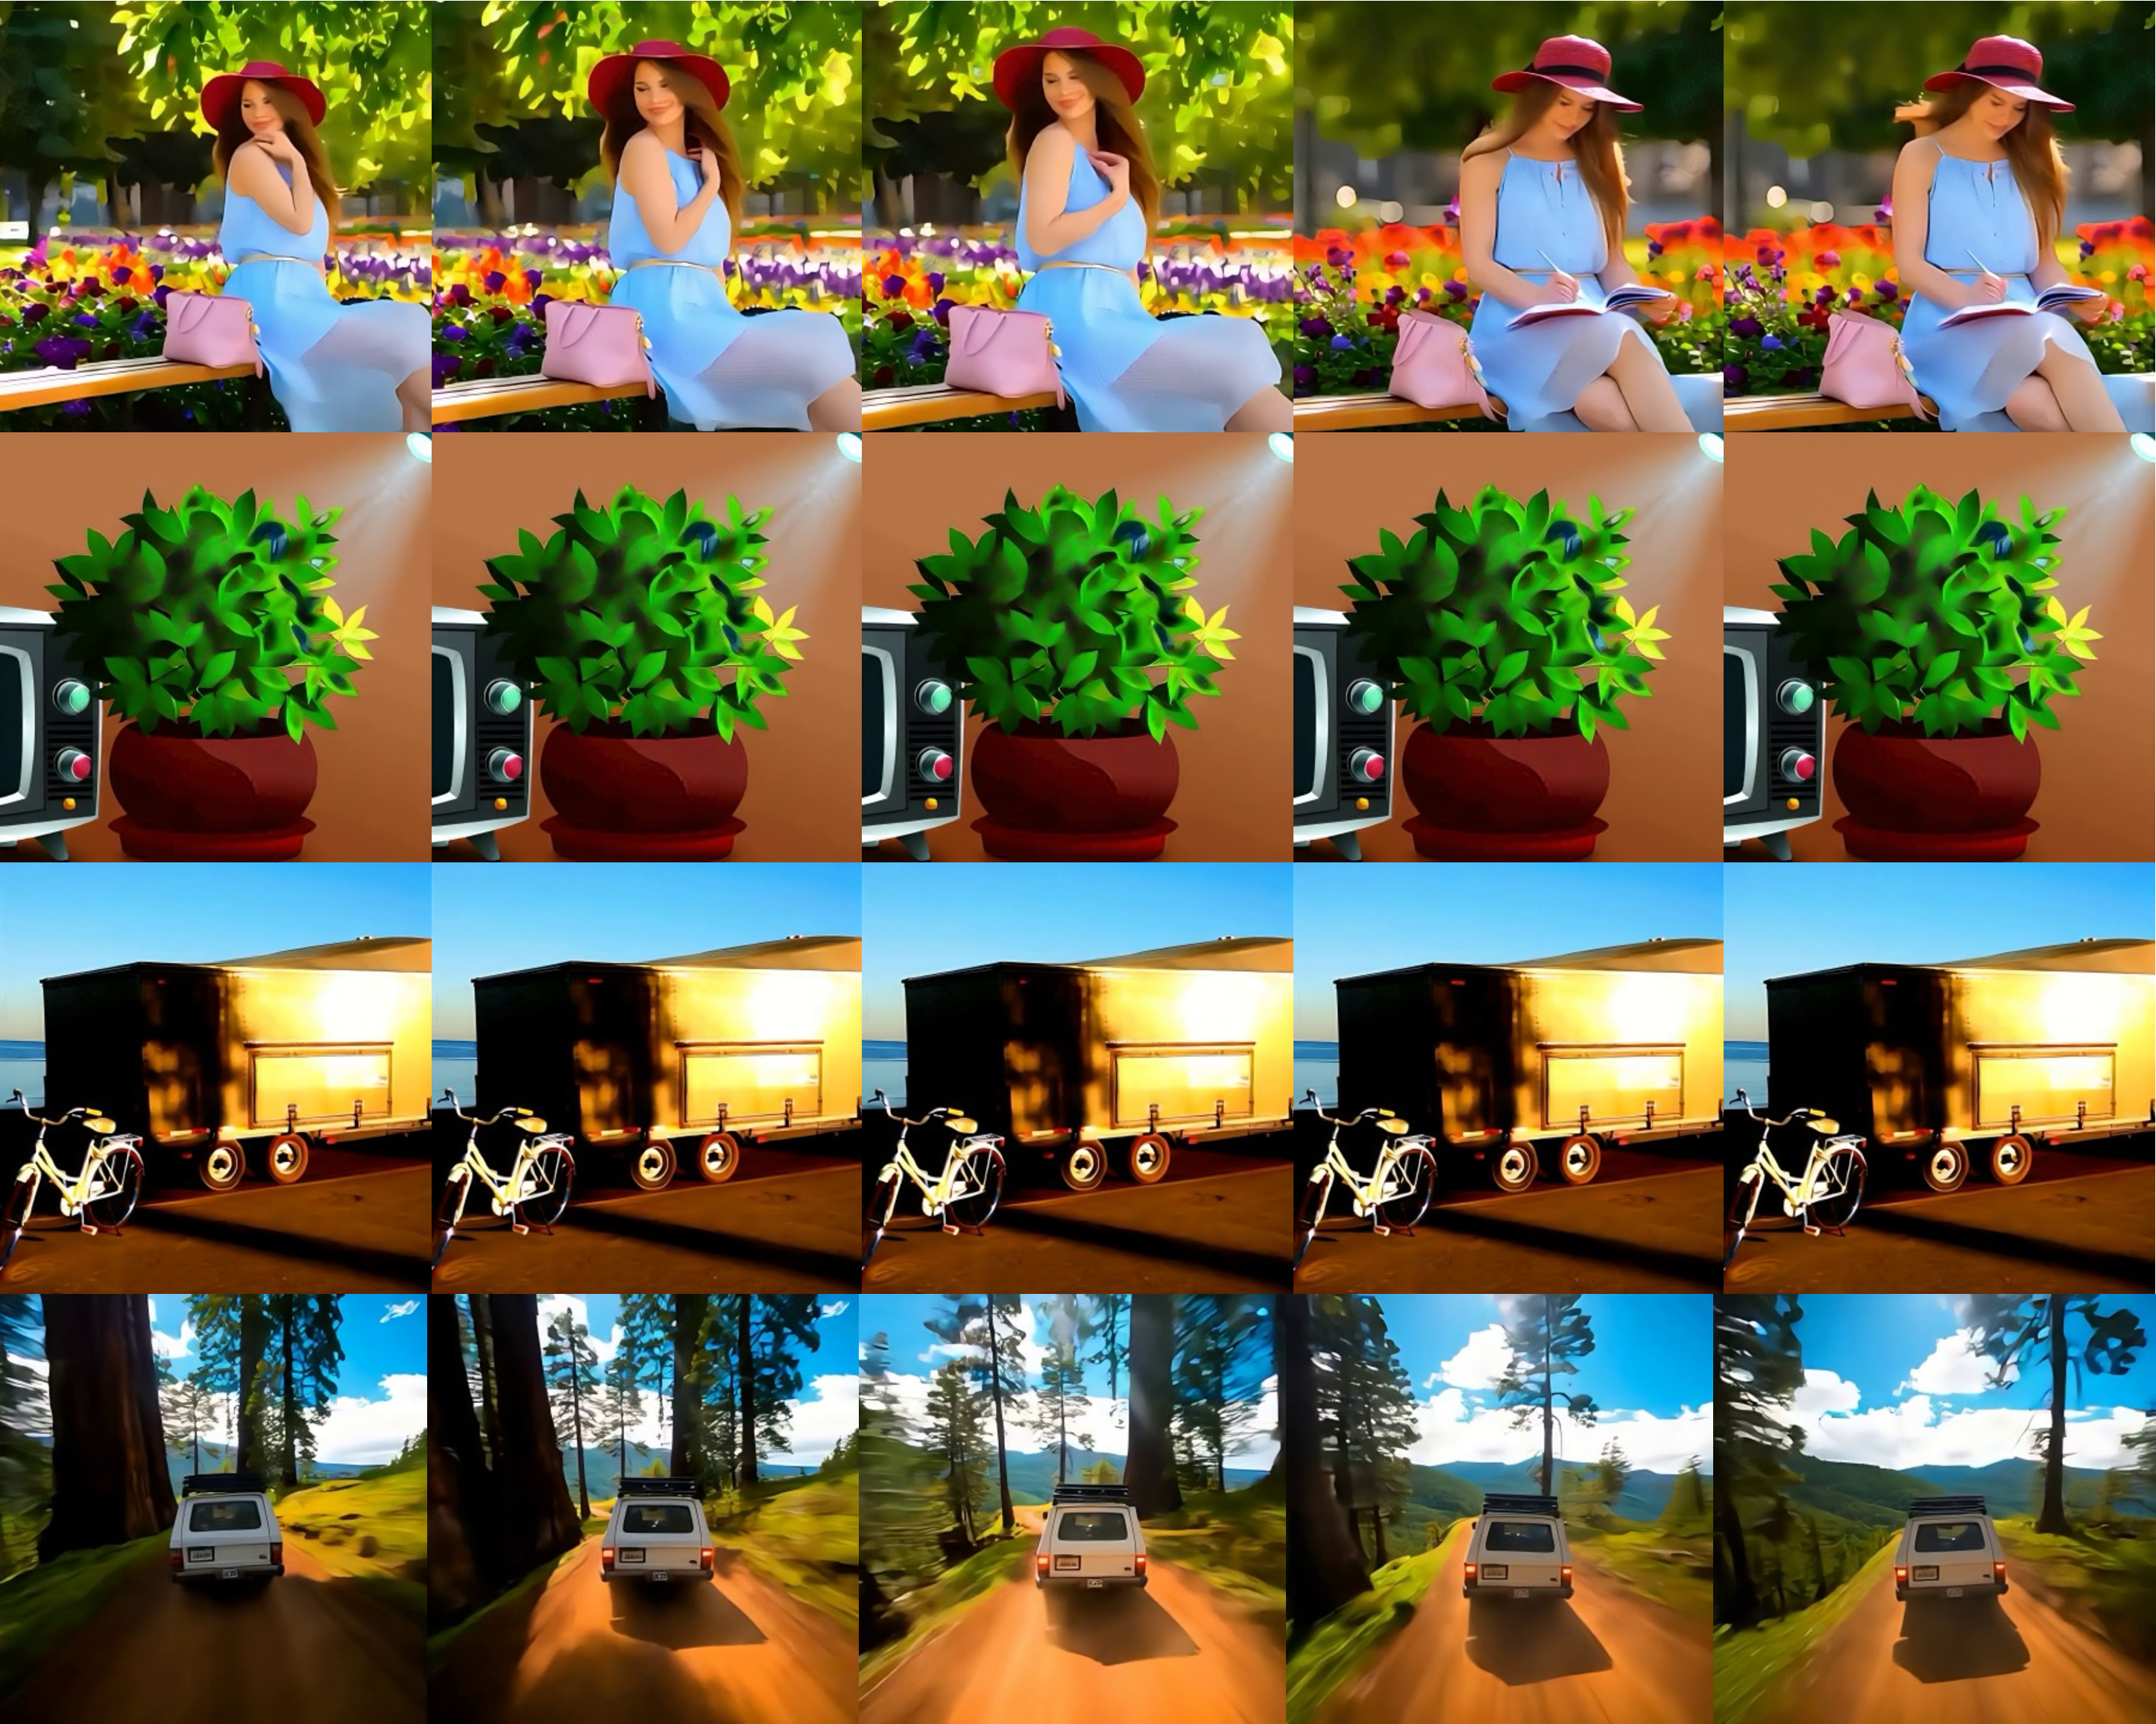
\includegraphics[width=\textwidth]{final/RealBasicVSR.pdf}
        \caption{RealBasicVSR方法}
        \label{fig:rbvsr}
    \end{subfigure}
    \hfill
    \begin{subfigure}[b]{0.3\textwidth}
        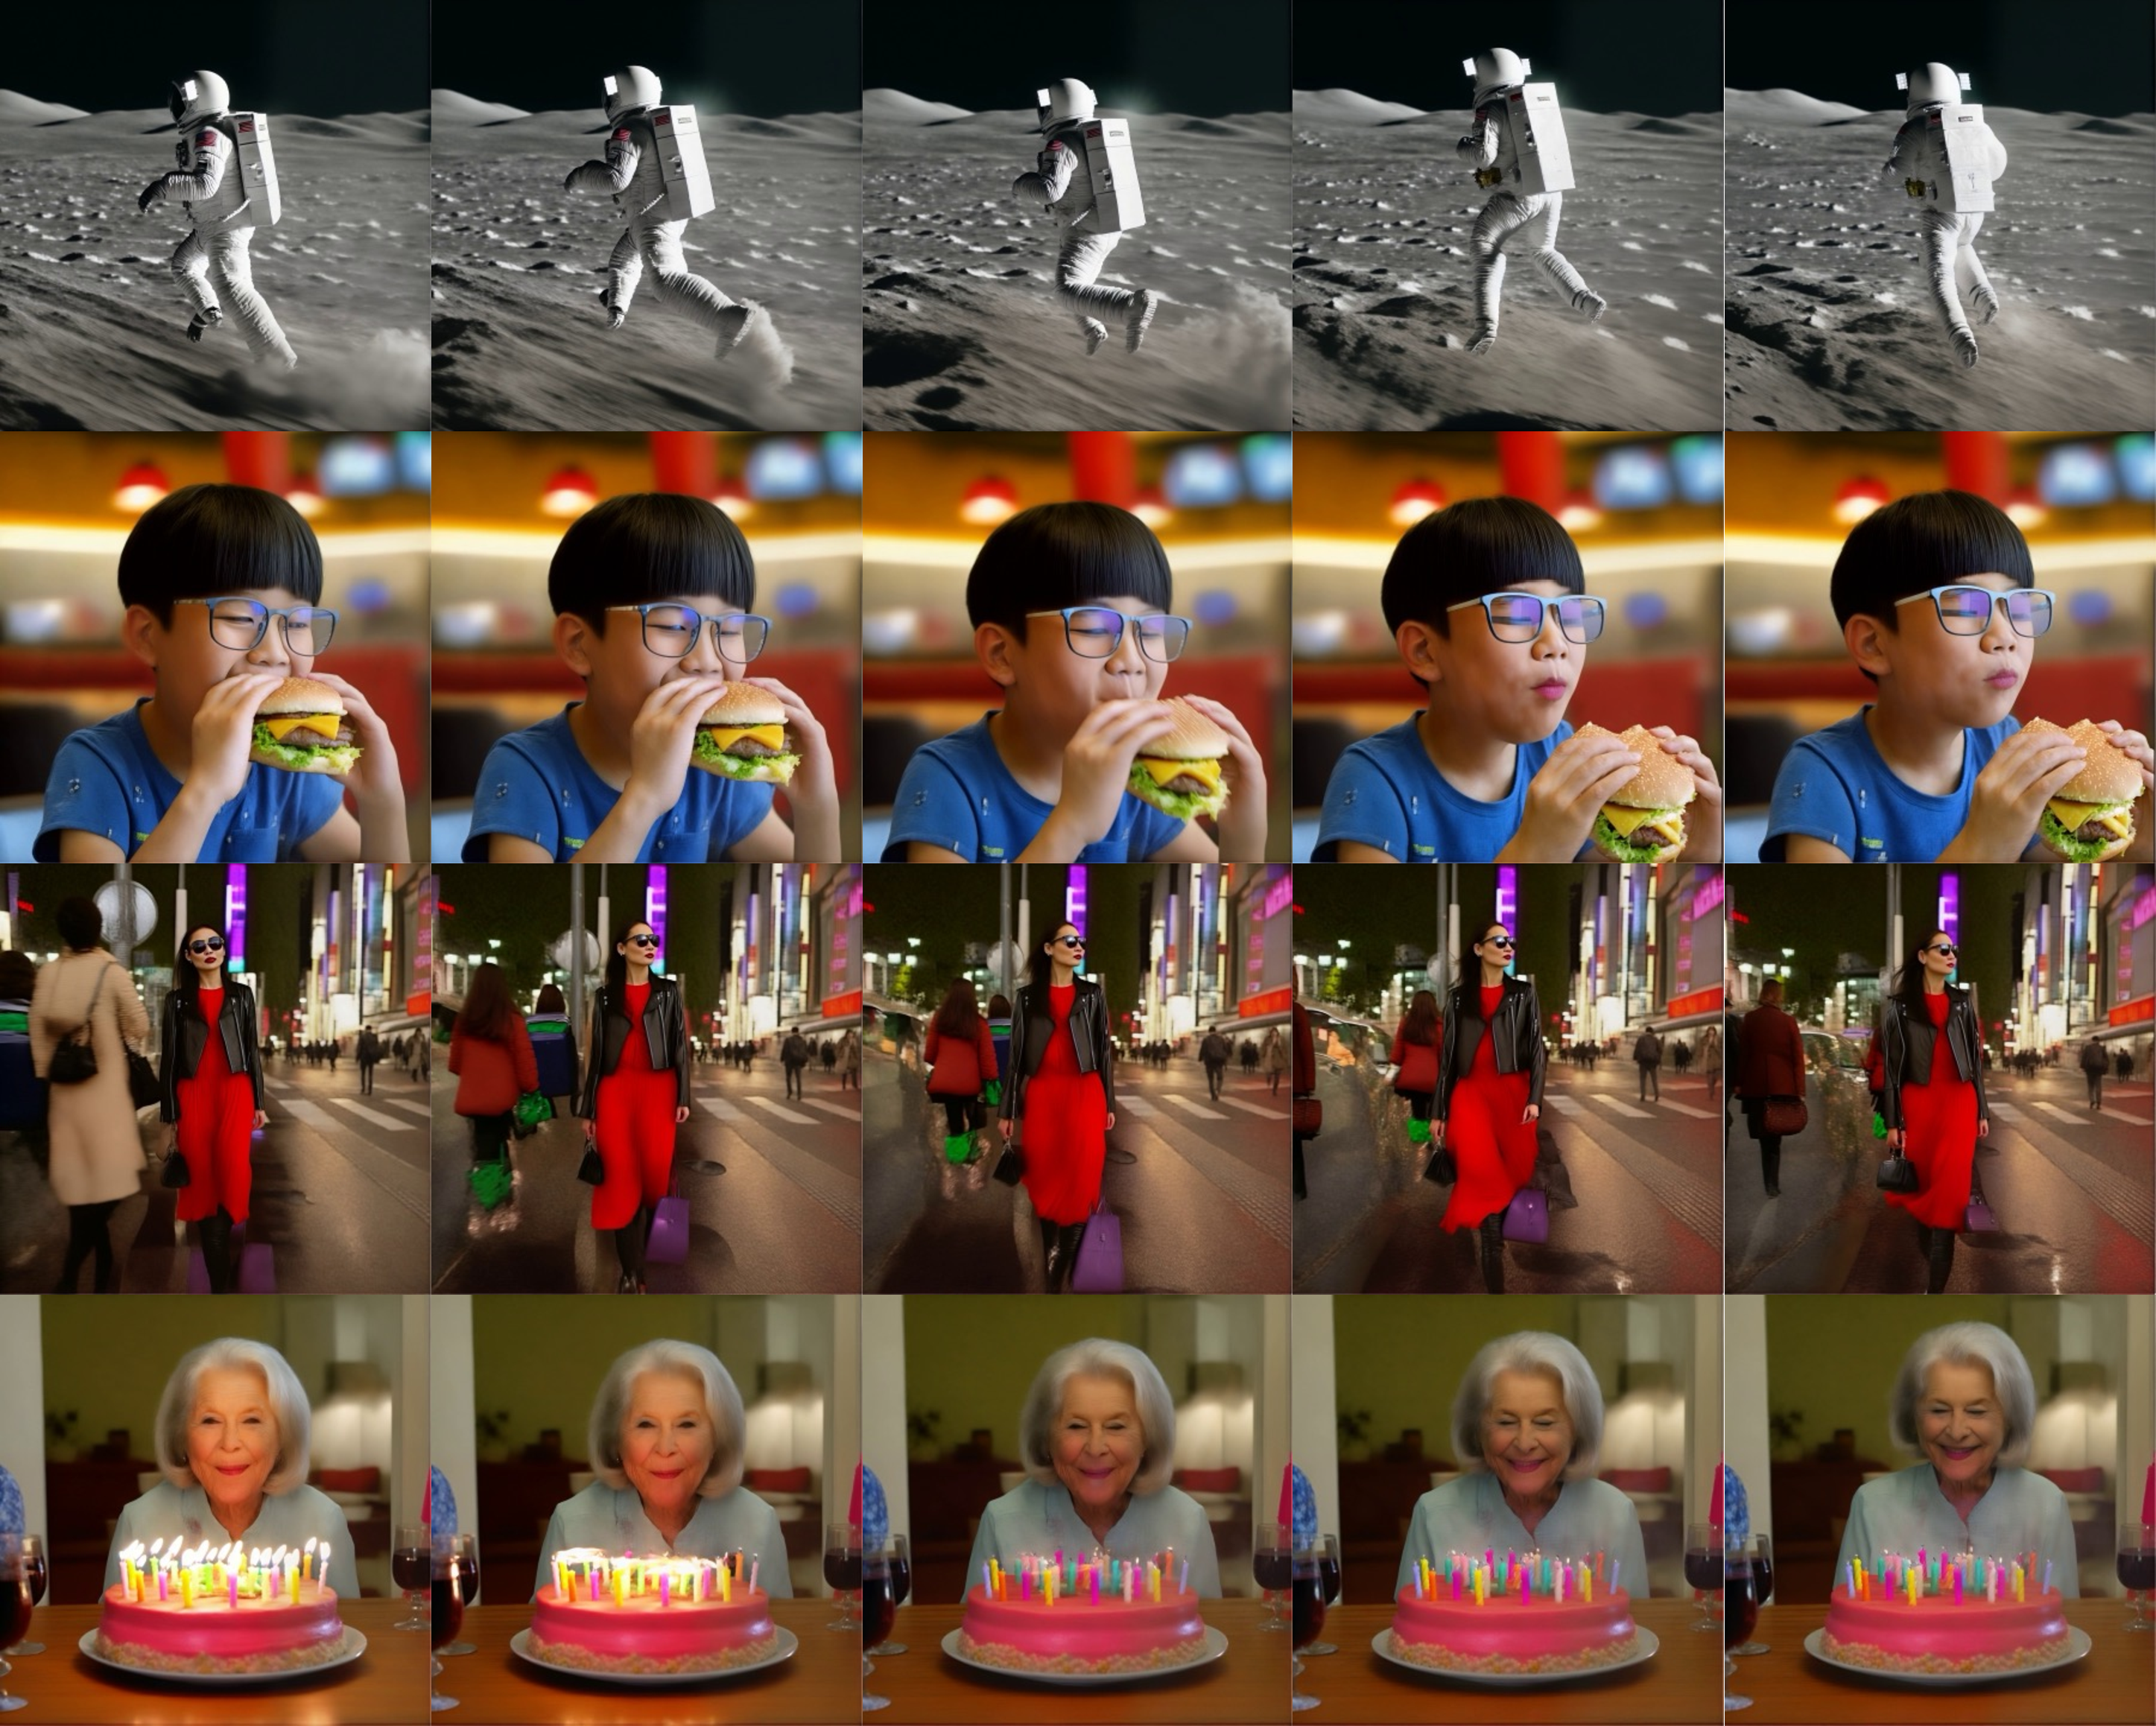
\includegraphics[width=\textwidth]{final/VEnhancer.pdf}
        \caption{VEnhancer}
        \label{fig:venhancer方法}
    \end{subfigure}

    \caption{不同视频超分方法结果展示。(a)为我们的实验结果,(b)为Upscale-A-Video方法, (c)为RealBasicVSR方法结果,(d)为VEnhancer实验结果。放大观看效果更佳。}
    \label{fig:vsrcompare}
\end{figure}



\subsection{本章小结}
本章详细呈现并深入分析了第三章所设计的实验结果。首先,明确了研究所采用的评估方法,包括VBench等常用图像和视频质量评估指标,并解释了其实现方式和评估作用。随后,从定性和定量两个维度,对针对参考图可控视频生成方法(包含两种实验设置)和高分辨率参考图视频生成方法的实验结果进行了多方面分析,并与其他SOTA方法进行了优劣比较。

\section{未来展望}
本文围绕基于参考图像的视频生成技术展开了系统性的研究与探索。
首先,本文对两种核心的参考图可控视频生成训练策略——首帧潜变量替换与参考帧潜变量拼接进行了详细的实现与对比分析,明确了首帧替换策略在动作幅度和语义保持方面的优势及其更快的收敛特性。

其次,针对视频中特定主体身份信息保持的挑战,本章提出了一种改进的ID注入方法。该方法通过对参考图像潜变量的灵活拼接与对位置编码约束的调整,成功实现了在保持核心ID信息的同时,赋予生成视频更自然、更多样的动态表现。VBench定量评估结果亦证实了该方法在主体一致性和运动平滑性上的优越性。

最后,为攻克给定高分辨率图片生成对于分辨率视频带来的巨大计算瓶颈,本章引入并实现了一种基于流匹配的高效生成方案。该方案采用轻量级预训练模型,并借鉴flowing matching“走直线”的核心思想,通过优化潜变量的转换路径与迭代方式,显著提升了高分辨率视频的生成效率。与现有主流模型的对比实验充分证明了本方法在推理速度上的巨大优势,使其在资源受限条件下生成高分辨率视频成为可能。

并且为更好地评估生成视频的质量,本文从定性与定量两个维度,对三种不同设置下的实验结果进行了多方面分析,并构建了一个包含108个视频文本描述的测试集,涵盖人物、动物、物体和风景等多个类别。


综上所述,本章的研究工作为实现高质量、高一致性且高效率的参考图像引导视频生成提供了多方面的技术改进和实践方案,为后续的视频内容创作与应用奠定了坚实的基础。

尽管本文基于参考图像的视频生成技术做了相应的调研及实验,但仍存在进一步改进和拓展的空间:
当前系统主要基于单一参考图像进行视频生成,未来可探索融合视频,音频等多模态输入的控制机制。特别是引入视频描述作为辅助引导,有望实现更细粒度的运动控制和语义表达。此外,研究如何将用户交互(如草图、关键点标注)整合到生成流程中,将显著提升系统的实用性和可控性。之后研究更大的数据集上进行测试,观察目前研究方案在世界真实场景下是否具有泛化性。
此外现有方法在短时视频(通常5秒左右)生成中表现良好,但对于更长时序的视频(30秒以上),仍面临严重的身份漂移和场景突变问题。未来工作可通过修改位置编码等training-free方式或者修改模型架构以适应长序列建模方式, 逐步构建更长的视频生成世界, 做到用生成的视频去真实的模拟现实世界场景,以期为未来世界模型的诞生奠定基础。
